\documentclass[conference]{IEEEtran}

\usepackage[utf8]{inputenc}
\usepackage[T1]{fontenc}
\usepackage[turkish,shorthands=:!]{babel}
\usepackage{amsmath,amssymb}
\usepackage{graphicx}
\usepackage{booktabs}
\usepackage{multirow}
\usepackage{cite}
\usepackage{url}
\usepackage[hidelinks]{hyperref}

\graphicspath{{figures/}}

\begin{document}

\renewcommand{\IEEEkeywordsname}{Anahtar Kelimeler}

\title{Makine Öğrenmesi Tabanlı Saldırı Tespit Sistemlerinin Adversarial Evasion Saldırılarına Karşı Dayanıklılığının Değerlendirilmesi}

\author{\IEEEauthorblockN{Ömer Faruk Sayın}
\IEEEauthorblockA{Bilgisayar Mühendisliği Anabilim Dalı, Yüksek Lisans\\
Kırşehir Ahi Evran Üniversitesi, Kırşehir, Türkiye\\
sayinfaruk2002@gmail.com}}

\maketitle

\begin{abstract}
Makine öğrenmesi tabanlı saldırı tespit sistemleri (IDS) standart test verisinde neredeyse kusursuz sonuçlar verebilmektedir. Bu çalışmada, saldırganın kendi trafiğini küçük ve gerçekçi ölçülerde değiştirmesi durumunda bu başarının ne ölçüde korunduğu incelenmiştir. CIC-IDS2017 üzerinde Random Forest, XGBoost ve MLP modelleri eğitilmiş; test kümesindeki saldırı akışları ağ trafiğinin temel kısıtlarını koruyan bir pertürbasyonla değiştirilmiştir. Saldırgan yalnızca kendi gönderdiği paketlere dolgu ekleyebilmekte ve gönderimi geciktirebilmektedir; türetilmiş özellikler yeniden hesaplanmaktadır. Rastgele bir saldırgan, model skorunu sorgulayan gradyansız bir uyarlamalı saldırganla karşılaştırılmıştır. Temiz veride F1 değerleri 0.987--0.998 arasındadır. Uyarlamalı saldırgan, boyut ve zamanı \%50'ye kadar artırarak Random Forest'ın kaçırdığı saldırı sayısını 281'den 5\,479'a çıkarmaktadır. Buna karşın sıralama kalitesi büyük ölçüde korunmaktadır (PR-AUC $\geq 0.992$). Nitekim eşik yalnızca doğrulama verisiyle ve \%0.1'lik bir yanlış alarm bütçesine göre seçildiğinde Random Forest'ın saldırı altında kaçırdığı saldırılar \%77 azalmakta, olasılık kalibrasyonu ise tek başına bir iyileşme sağlamamaktadır. Yavaş DoS akışlarının yaklaşık \%40'ı yalnızca \%5'lik bir gecikmeyle tespitten kaçmaktadır. Deney CSE-CIC-IDS2018 üzerinde tekrarlandığında dayanıklılık sıralaması değişmekte; 2017'de göreli kayba göre en dayanıklı model olan MLP, 2018'de en kırılgan model olmaktadır. İki veri setinde de istikrarlı kalan tek model XGBoost'tur.
\end{abstract}

\begin{IEEEkeywords}
saldırı tespit sistemleri, adversarial makine öğrenmesi, evasion saldırıları, dayanıklılık, karar eşiği, CIC-IDS2017, CSE-CIC-IDS2018
\end{IEEEkeywords}

\section{Giriş}

Ağ tabanlı saldırı tespit sistemlerinde makine öğrenmesi modelleri, akış istatistiklerinden (paket boyutları, varış aralıkları, bayrak sayıları) saldırıyı normal trafikten ayırmayı öğrenir. CIC-IDS2017 gibi kamuya açık veri setlerinde ağaç tabanlı modellerin F1 değerlerinin 0.99'un üzerine çıkması artık olağan bir sonuçtur. Ancak bu değerler modelin \emph{rastgele seçilmiş} test akışlarındaki başarısını ölçer; tespit edilmemeye çalışan bir saldırgan karşısındaki davranışı hakkında doğrudan bilgi vermez.

Adversarial makine öğrenmesi literatürü, girdide yapılan küçük ve hedefli değişikliklerin yüksek doğruluklu modelleri yanıltabildiğini uzun süredir göstermektedir \cite{szegedy2014,goodfellow2015,biggio2013}. Ne var ki bu sonuçların büyük kısmı görüntü alanından gelmektedir ve ağ trafiğine olduğu gibi aktarılamaz: bir pikselin değeri serbestçe değiştirilebilirken bir akışın paket sayısı, süresi ve bayt hızı birbirine bağlıdır ve saldırgan bunların yalnızca bir kısmını kontrol edebilir. Apruzzese ve arkadaşları, ağ IDS'leri üzerine yapılan adversarial çalışmaların önemli bir kısmının gerçekçi olmayan saldırgan varsayımlarına dayandığını vurgulamaktadır \cite{apruzzese2022}. Kısıt gözetmeyen bir pertürbasyon, modelin kırılganlığını olduğundan büyük gösterebilir.

Ağ IDS'leri üzerine yapılan çalışmaların önemli bir kısmında üç ortak eksiklik göze çarpmaktadır. Birincisi, pertürbasyon çoğunlukla standartlaştırılmış özellik uzayında tanımlanmaktadır; bu durumda aynı $\varepsilon$ bir özellikte birkaç bayta, başka bir özellikte saniyelere karşılık gelebilmekte ve türetilmiş özellikler (hızlar, ortalamalar) değiştirilen özelliklerle tutarsız kalabilmektedir. İkincisi, gradyan tabanlı saldırılar ağaç modellerine doğrudan uygulanamadığından modeller çoğu zaman aynı saldırgan altında karşılaştırılamamaktadır. Üçüncüsü, sonuçlar genellikle tek bir veri setinde ve sabit bir karar eşiğiyle raporlanmaktadır; bu da gözlenen kırılganlığın modele mi, veri setine mi, yoksa eşik seçimine mi ait olduğunu ayırt etmeyi güçleştirmektedir. Bu çalışma bu üç noktayı doğrudan ele alacak biçimde tasarlanmıştır.

Çalışmanın araştırma sorusu şudur: \emph{Gerçekçi ağ kısıtları altında yapılan adversarial pertürbasyonlar ML tabanlı IDS modellerinin performansını ne ölçüde düşürmektedir ve hangi model bu değişikliklere daha dayanıklıdır?} Sınanan hipotez ise şöyledir. \textbf{H1}: Pertürbasyon seviyesi arttıkça saldırı sınıfına ilişkin Recall ve F1 değerleri düşmektedir.

Çalışmanın katkıları aşağıda özetlenmiştir:
\begin{enumerate}
\item \textbf{Kısıtları açıkça doğrulanan bir pertürbasyon çerçevesi.} Pertürbasyon ölçeklenmiş uzayda değil, ham birimlerde göreli bir bütçe ($\varepsilon$) olarak tanımlanmıştır. Saldırgan yalnızca ileri yöndeki paket boyutlarını ve zamanlamayı artırabilmektedir; hız ve çift yönlü ortalamalar gibi türetilmiş özellikler yeniden hesaplanmakta ve değerler eğitim aralığında tutulmaktadır. Yedi kısıtın sağlandığı her çalıştırmada otomatik olarak sınanmaktadır.
\item \textbf{Saldırgan bilgisinin katkısının ayrıştırılması.} Gradyan gerektirmeyen ve yalnızca model skorunu sorgulayan uyarlamalı bir saldırgan, ağaç tabanlı modellerle sinir ağının aynı koşullarda karşılaştırılmasını mümkün kılmaktadır. Aynı bütçeyle çalışan rastgele saldırgan ise kaybın ne kadarının saldırganın modeli hedeflemesinden kaynaklandığının ayrıştırılmasını sağlamaktadır.
\item \textbf{Saldırı türü ve özellik grubu düzeyinde hata analizi.} Yavaş DoS saldırılarının sabit bir süre imzasıyla tanındığı ve küçük bir gecikmeyle tespitten kaçtığı, saldırganın değiştiremediği sayaç ve protokol özelliklerinin ise dayanıklılığa en fazla katkı yapan grup olduğu gösterilmiştir.
\item \textbf{İkinci bir veri setinde tekrar.} Aynı 64 özellikle CSE-CIC-IDS2018 üzerinde yapılan tekrar, model dayanıklılık sıralamasının veri setindeki saldırı bileşimine bağlı olduğunu ve tek bir veri setinden genellenemeyeceğini ortaya koymaktadır.
\item \textbf{Karar eşiğinin dayanıklılıktaki payının ölçülmesi.} Eşik ve kalibrasyon parametreleri yalnızca doğrulama verisiyle seçildiğinde, saldırı altındaki kaybın önemli bir kısmının skorların sabit 0.5 eşiğinin hemen altına inmesinden kaynaklandığı ve kalibrasyonun bu kaybı tek başına azaltmadığı gösterilmiştir.
\end{enumerate}

\section{İlgili Çalışmalar}

\subsection{Adversarial makine öğrenmesi}
Biggio ve arkadaşları test anında yapılan evasion saldırılarını gradyan tabanlı bir optimizasyon problemi olarak tanımlamıştır \cite{biggio2013}. Szegedy ve arkadaşları derin ağların algılanamayacak kadar küçük pertürbasyonlarla yanıltılabildiğini göstermiş \cite{szegedy2014}, Goodfellow ve arkadaşları ise bu örnekleri tek adımda üreten FGSM yöntemini önermiştir \cite{goodfellow2015}. Biggio ve Roli alanın on yıllık gelişimini tehdit modelleri üzerinden özetlemektedir \cite{biggio2018}. Bu yöntemler modelin gradyanına ihtiyaç duyar. Karar ağaçları ve topluluk modelleri türevlenebilir olmadığından Kantchelian ve arkadaşları ağaç toplulukları için ayrı saldırı ve sağlamlaştırma yöntemleri geliştirmiştir \cite{kantchelian2016}. Yalnızca modelin çıktısına erişen kara kutu saldırılar da bu sınırlamayı aşar; HopSkipJump gibi karar tabanlı yöntemler yalnızca etiket sorgularıyla çalışır \cite{chen2020}.

\subsection{Ağ IDS'lerine yönelik adversarial saldırılar}
Ağ trafiğinde saldırının iki düzeyde yapılabileceği kabul edilmektedir: özellik uzayında, yani akış özellikleri doğrudan değiştirilerek, ya da problem uzayında, yani paketler yeniden üretilerek. Özellik uzayındaki çalışmalar uygulanabilirlik açısından sıklıkla eleştirilmektedir; değiştirilen özelliklerin gerçek bir akışa karşılık gelip gelmediği, saldırganın o özelliği kontrol edip edemediği ve saldırının işlevini koruyup korumadığı çoğu zaman sınanmamaktadır \cite{apruzzese2022}. Pierazzi ve arkadaşları problem uzayındaki saldırılar için uygulanabilir dönüşümler, anlamın korunması ve inandırıcılık gibi kısıtları biçimsel olarak tanımlamıştır \cite{pierazzi2020}. Sheatsley ve arkadaşları ağ verisinin alan kısıtlarını hesaba katan saldırıların da IDS modellerini yanıltabildiğini göstermiştir \cite{sheatsley2022}. Alhajjar ve arkadaşları ise adversarial örnekleri evrimsel yöntemler ve üretici çekişmeli ağlarla üretmiştir \cite{alhajjar2021}. Rosenberg ve arkadaşları siber güvenlik alanındaki saldırı ve savunma yöntemlerini kapsamlı biçimde derlemektedir \cite{rosenberg2021}; savunma tarafında en yaygın yaklaşım pertürbe edilmiş örneklerle eğitimdir \cite{madry2018}. Bu çalışma özellik uzayında kalmakla birlikte saldırganın kontrol alanını açıkça sınırlamakta, türetilmiş özellikleri tutarlı biçimde güncellemekte ve gradyan gerektirmeyen bir saldırganla üç modeli aynı koşullarda karşılaştırmaktadır.

\subsection{Olasılık kalibrasyonu ve karar eşiği}
Bir sınıflandırıcının ürettiği skorun gerçek bir olasılık gibi yorumlanabilmesi için kalibre olması gerekir. Niculescu-Mizil ve Caruana, farklı öğrenme yöntemlerinin olasılık kalitesini karşılaştırarak topluluk modellerinin ve boosting'in sistematik biçimde kalibre olmayan skorlar üretebildiğini göstermiştir \cite{niculescu2005}. Bu skorları düzeltmek için Platt scaling \cite{platt1999}, isotonic regression \cite{zadrozny2002} ve sinir ağları için temperature scaling \cite{guo2017} kullanılmaktadır. IDS çalışmalarında karar eşiği çoğunlukla 0.5'te sabit bırakılmakta, adversarial dayanıklılığın bu seçime ne kadar bağlı olduğu ise nadiren incelenmektedir.

\subsection{Veri setleri ve değerlendirme tuzakları}
CIC-IDS2017 ve CSE-CIC-IDS2018, aynı akış çıkarıcıyla (CICFlowMeter) laboratuvar ortamında üretilmiş, etiketli ve yaygın kullanılan iki veri setidir \cite{sharafaldin2018}. Engelen ve arkadaşları CIC-IDS2017'de akış üretimi ve etiketleme hatalarını raporlamış \cite{engelen2021}, Liu ve arkadaşları benzer hataların CSE-CIC-IDS2018'de de bulunduğunu göstermiştir \cite{liu2022}. Sommer ve Paxson IDS'lerde makine öğrenmesinin laboratuvar dışına taşınmasının zorluklarını \cite{sommer2010}, Arp ve arkadaşları ise güvenlik alanındaki makine öğrenmesi çalışmalarında sık görülen veri sızıntısı ve sahte korelasyon gibi tuzakları tartışmaktadır \cite{arp2022}. Bu uyarılar doğrultusunda bu çalışmada sızıntı kontrolleri ayrı bir adım olarak raporlanmıştır.

\section{Veri Setleri ve Ön İşleme}

\subsection{CIC-IDS2017}
MachineLearningCVE sürümünün sekiz günlük dosyası birleştirilmiştir (2\,830\,743 akış, 79 sütun). Temizlik adımları sırasıyla şunlardır: sonsuz değerlerin eksik değere çevrilip eksik satırların atılması (2\,867 satır), fiziksel olarak geçersiz negatif değerli satırların atılması (2\,925 satır; \texttt{Init\_Win\_bytes} sütunlarındaki $-1$ ``gözlenmedi'' anlamına geldiği için bu kuraldan muaftır), 8 sabit ve 5 kopya sütunun silinmesi, aynı özelliklere sahip olup hem normal hem saldırı etiketi taşıyan 82\,458 satırın atılması ve özellikleri birebir aynı 512\,705 satırın tekilleştirilmesi. \texttt{Destination Port} bir davranış değil tanımlayıcı olduğu için model özelliklerinden çıkarılmıştır. Sonuçta 2\,229\,788 akış ve 64 özellik kalmıştır; akışların \%15.07'si saldırıdır (14 saldırı türü).

\subsection{Sızıntı ve dengesizlik analizi}
Tekilleştirme sonrasında test kümesinde eğitim kümesiyle birebir aynı olan akış bulunmamaktadır (445\,958 test akışında 0). Hiçbir özellik tek başına 0.95'in üzerinde ROC-AUC vermemektedir; en yüksek değer \texttt{Fwd IAT Std} için 0.846'dır. Saldırı türleri belirli portlarda yoğunlaşsa da (ör. DoS saldırılarının tamamı port 80) port özellik olarak eklendiğinde XGBoost'un F1 değeri yalnızca 0.9975'ten 0.9983'e çıkmaktadır (seed 42, 400\,000 eğitim örneği). Bu kontroller yüksek başarının tek bir kısayola dayanmadığını göstermektedir. Sınıf oranı 5.6:1'dir; her akışı ``normal'' olarak sınıflandıran bir model 0.849 doğruluk elde eder. Bu nedenle değerlendirme saldırı sınıfının Recall, F1, PR-AUC ve yanlış negatif (FN) değerlerine odaklanmaktadır; yeniden örnekleme yapılmamıştır.

\subsection{CSE-CIC-IDS2018}
Resmî kaynaktaki on günlük dosyanın dokuzu kullanılmıştır. 3.9~GB boyutundaki 20-02-2018 günü (yalnızca DDoS-LOIC-HTTP) boyutu nedeniyle dışarıda bırakılmış; DDoS saldırıları HOIC ve LOIC-UDP ile temsil edilmiştir. Kısaltılmış sütun adları 2017'deki karşılıklarına eşlenmiş ve aynı 64 özellik kullanılmıştır. Bellek sınırı nedeniyle her dosyadan \%30 oranında rastgele örnek alınmış (2\,485\,256 akış); aynı temizlik adımlarından sonra 1\,734\,219 akış kalmıştır (\%15.13 saldırı). 2018 verisi bağımsız bir tekrar olarak kullanılmıştır: modeller 2018 verisinin kendi eğitim kümesiyle eğitilmiş ve kendi test kümesinde değerlendirilmiştir. 2017'de eğitilen modeller 2018 verisinde test edilmemiştir; veri setleri arası genelleme bu çalışmanın kapsamı dışındadır. Tablo~\ref{tab:data} iki veri setini özetlemektedir.

\begin{table}[t]
\caption{Kullanılan veri setlerinin özeti}
\label{tab:data}
\centering
\begin{tabular}{lrr}
\toprule
 & CIC-IDS2017 & CSE-CIC-IDS2018 \\
\midrule
Ham / örneklem akış & 2\,830\,743 & 2\,485\,256 \\
Temizlik sonrası akış & 2\,229\,788 & 1\,734\,219 \\
Saldırı oranı & \%15.07 & \%15.13 \\
Saldırı türü sayısı & 14 & 13 \\
Testteki saldırı akışı & 67\,206 & 52\,483 \\
\bottomrule
\end{tabular}
\end{table}

\section{Yöntem}

\subsection{Modeller ve değerlendirme protokolü}
Üç farklı karar mantığını temsil eden üç model kullanılmıştır: 100 ağaçlı Random Forest (bagging), 200 ağaçlı XGBoost \cite{chen2016} (boosting; derinlik 8, öğrenme oranı 0.1, satır ve sütun örnekleme 0.8) ve 64--32 gizli katmanlı, erken durdurmalı bir MLP. Random Forest ve MLP için scikit-learn \cite{pedregosa2011} kütüphanesinden yararlanılmıştır. SVM çalışmaya dahil edilmemiştir: çekirdekli SVM'nin eğitim maliyeti örnek sayısıyla en az karesel olarak arttığından, yaklaşık 1.8 milyon eğitim akışı ve her seed için tekrarlanan eğitim düşünüldüğünde pratik değildir. Seçilen üç model bagging, boosting ve sinir ağı olmak üzere birbirinden farklı üç karar mantığını kapsamaktadır. Veri her seed için \%80/\%20 oranında katmanlı olarak bölünmüş, \texttt{StandardScaler} yalnızca eğitim kümesine uyarlanmıştır. Seed değerleri (42, 100, 2024) hem bölmeyi hem model başlangıcını hem de pertürbasyonun rastgeleliğini belirlemektedir. Sonuçlar üç seed üzerinden ortalama $\pm$ standart sapma olarak verilmiştir. Karar eşiği 0.5'tir. Hiperparametreler sabit tutulmuş, test verisi hiçbir ayar ya da seçim için kullanılmamıştır; MLP'nin erken durdurması eğitim kümesinden ayrılan \%10'luk doğrulama verisiyle yapılmıştır.

\subsection{Tehdit modeli}
Saldırganın yalnızca kendi saldırı akışlarını kontrol ettiği varsayılmıştır; normal trafik ve model değişmemektedir. Saldırgan kendi gönderdiği (ileri yön) paketlere dolgu ekleyebilir ve gönderimi geciktirebilir. Sunucu yanıtlarını değiştiremez, paket ekleyip çıkaramaz ve hiçbir değeri azaltamaz; paketleri kısaltmak saldırının yükünü bozar, zamanı kısaltmak ise ağın izin verdiğinden daha hızlı göndermek anlamına gelir.

\subsection{Kısıtlı pertürbasyon}
Ölçeklenmiş uzayda tanımlanan bir $\varepsilon$, çarpık dağılımlı özelliklerde birkaç bayta, diğerlerinde saniyelere karşılık gelebilir ve fiziksel olarak yorumlanamaz. Bu nedenle pertürbasyon ham birimlerde, göreli bir bütçeyle tanımlanmıştır. Her akış için bir boyut katsayısı $s \in [1, 1+\varepsilon]$ ve bir zaman katsayısı $t \in [1, 1+\varepsilon]$ seçilmektedir. İleri yöndeki yedi boyut özelliği (toplam, en küçük, en büyük, ortalama, standart sapma, segment ve alt akış baytı) $s$ ile, 23 zaman özelliği (süre, varış aralıkları, aktif ve boşta süreleri) $t$ ile çarpılmaktadır. Çift yönlü ortalamalar eklenen bayttan, hızlar ise yeni bayt miktarı ve yeni süreden yeniden hesaplanmaktadır:
\begin{equation}
\text{FlowBytes/s}' = \text{FlowBytes/s}\cdot\frac{B_{\text{fwd}}' + B_{\text{bwd}}}{B_{\text{fwd}} + B_{\text{bwd}}}\cdot\frac{1}{t}.
\end{equation}
Paket sayıları, bayraklar, başlık uzunlukları ve geri yön boyutları değişmemektedir. Katsayılar hiçbir özellik eğitim kümesindeki en büyük değeri aşmayacak şekilde sınırlanmakta ve tam sayı özellikler yuvarlanmaktadır. 20\,000 saldırı akışına en yüksek bütçe ($\varepsilon=1.0$) uygulandığında yedi kısıtın tamamı sağlanmaktadır: negatif değer oluşmamakta, değerler eğitim aralığında kalmakta, tam sayılar korunmakta, değişmemesi gereken özellikler değişmemekte, değerler yalnızca artmakta, min $\leq$ ortalama $\leq$ max sıralaması ve en büyük paket ilişkisi korunmaktadır.

\subsection{Saldırganlar}
\emph{Rastgele saldırgan} her akış için $s$ ve $t$ değerlerini $1+\mathcal{U}(0,\varepsilon)$ dağılımından çeker ve modeli tanımaz. \emph{Uyarlamalı saldırgan} modelin iç yapısını bilmez, ancak saldırı olasılığını sorgulayabilir. Her akış için $\{1, 1+\varepsilon/3, 1+2\varepsilon/3, 1+\varepsilon\}$ kümesinden seçilen katsayıları (boyut ve zaman birlikte değiştirildiğinde 16 kombinasyon) dener ve saldırı olasılığını en düşük yapan seçeneği kullanır. Gradyana ihtiyaç duymadığı için üç modele aynı biçimde uygulanabilir.

\subsection{Deneyler ve istatistiksel analiz}
Deney A temiz test verisinde baseline performansı ölçer. Deney B iki saldırgan, üç özellik grubu (boyut, zaman ve ikisi birlikte) ve altı bütçe ($\varepsilon \in \{0, 0.05, 0.10, 0.25, 0.50, 1.00\}$) için performansı ölçer. Deney C modelleri karşılaştırır; \emph{dayanıklılık skoru} $\varepsilon>0$ seviyelerindeki $F1_\varepsilon / F1_0$ oranlarının ortalamasıdır. Deney D özellik önemini ve özellik grubu ablasyonunu (grup çıkarılıp model 400\,000 örnekle yeniden eğitilerek) inceler. H1, her model, saldırgan ve grup kombinasyonu için $\varepsilon$ ile Recall ve F1 arasındaki Spearman sıra korelasyonuyla sınanmıştır (6 bütçe $\times$ 3 seed $=$ 18 gözlem; $\rho<0$, $p<0.05$). Bir kombinasyonda H1'in desteklenmiş sayılması için iki testin de anlamlı olması gerekmektedir. Her veri setinde 18 kombinasyonda toplam 36 test yapıldığından Holm düzeltmesi de raporlanmıştır. Ana karşılaştırmalar için seedler üzerinden t dağılımına dayalı \%95 güven aralıkları (GA) hesaplanmıştır.

\subsection{Karar eşiği ve kalibrasyon analizi}
Saldırı altında PR-AUC korunurken Recall'un düşmesinin eşik seçimiyle ilişkisini sınamak için ek bir analiz yapılmıştır. Aynı test bölmesi korunarak her seed'in eğitim kümesinden \%10'luk bir doğrulama kümesi ayrılmış ve modeller kalan \%90 ile yeniden eğitilmiştir. Eşikler ve kalibrasyon parametreleri yalnızca bu doğrulama kümesinde belirlenmiş, test verisi hiçbir seçim için kullanılmamıştır. Üç eşik politikası karşılaştırılmıştır: sabit 0.5, doğrulamada F1'i en yüksek yapan eşik ve doğrulamada yanlış alarm oranını \%0.1 ile sınırlayan en düşük eşik. Kalibrasyon için Platt scaling, isotonic regression ve (logit çıktısı anlamlı olan XGBoost ve MLP için) temperature scaling uygulanmış; Brier skoru, beklenen kalibrasyon hatası (ECE, 15 aralık) ve log-loss raporlanmıştır. Üç kalibrasyon yöntemi de skor sırasını koruyan dönüşümler olduğundan ROC-AUC ve PR-AUC'yi değiştirmez; uyarlamalı saldırgan da skoru en aza indirdiği için seçtiği pertürbasyon kalibrasyondan etkilenmez. Saldırı altındaki değerlendirme referans senaryoda (uyarlamalı, boyut+zaman, $\varepsilon=0.5$) yapılmıştır.

\subsection{Uygulama ve tekrarlanabilirlik}
Deneyler Python 3.14, scikit-learn 1.9, XGBoost 3.4, pandas 3.0 ve NumPy 2.4 ile, Intel Core i5-11400H işlemcili ve 16~GB bellekli bir dizüstü bilgisayarda yapılmıştır. Kod dört Jupyter notebook'undan oluşmaktadır: \path{00_cicids2017_robustness_experiments} (CIC-IDS2017, Deney A--D), \path{01_csecicids2018_replication_comparison} (CSE-CIC-IDS2018 ve karşılaştırma), \path{02_statistical_analysis} (Holm düzeltmesi ve güven aralıkları) ve \path{03_threshold_calibration_error_analysis} (eşik, kalibrasyon, hata analizi ve çıkarım süresi). Bütün rastgelelik kaynakları seed ile sabitlenmiştir; ham veri dışındaki bütün tablolar ve şekiller bu notebook'lar çalıştırıldığında yeniden üretilmektedir. Ham veri setleri boyutları nedeniyle depoya eklenmemiştir; resmî kaynaklardan nasıl indirileceği depodaki açıklama dosyasında verilmektedir.

\section{Sonuçlar}

\subsection{Baseline performansı (Deney A)}
Tablo~\ref{tab:baseline} temiz test verisindeki sonuçları göstermektedir. XGBoost en yüksek F1 değerine ve en az kaçırılan saldırı sayısına (157) sahiptir. MLP'nin Recall değeri ağaç modellerinden belirgin biçimde düşüktür; kaçırdığı saldırı sayısı XGBoost'un yaklaşık yedi katı, yanlış alarm sayısı ise yaklaşık altı katıdır. Seedler arasındaki standart sapmalar küçüktür. Sınıf dengesizliği nedeniyle doğruluk değerleri modeller arasındaki farkı gizlemektedir: en zayıf model olan MLP bile 0.996 doğruluğa sahiptir. Şekil~\ref{fig:cm} temiz veride ve referans saldırı senaryosunda karışıklık matrislerini göstermektedir; saldırı altında yalnızca sol alt hücre (kaçırılan saldırılar) değişmektedir.

\begin{table*}[t]
\caption{CIC-IDS2017, temiz test verisi (3 seed, ortalama $\pm$ std; FN ve FP seed ortalaması)}
\label{tab:baseline}
\centering
\small
\setlength{\tabcolsep}{4pt}
\begin{tabular}{lccccccrr}
\toprule
Model & Accuracy & Precision & Recall & F1 & ROC-AUC & PR-AUC & FN & FP \\
\midrule
Random Forest & 0.9991 $\pm$ 0.0001 & 0.9984 $\pm$ 0.0000 & 0.9958 $\pm$ 0.0004 & 0.9971 $\pm$ 0.0002 & 1.0000 & 0.9999 & 281 & 106 \\
XGBoost & 0.9994 $\pm$ 0.0000 & 0.9983 $\pm$ 0.0002 & 0.9977 $\pm$ 0.0003 & 0.9980 $\pm$ 0.0001 & 1.0000 & 1.0000 & 157 & 112 \\
MLP & 0.9961 $\pm$ 0.0004 & 0.9896 $\pm$ 0.0019 & 0.9844 $\pm$ 0.0009 & 0.9870 $\pm$ 0.0014 & 0.9997 & 0.9988 & 1\,051 & 694 \\
\bottomrule
\end{tabular}
\end{table*}

\begin{figure*}[t]
\centering
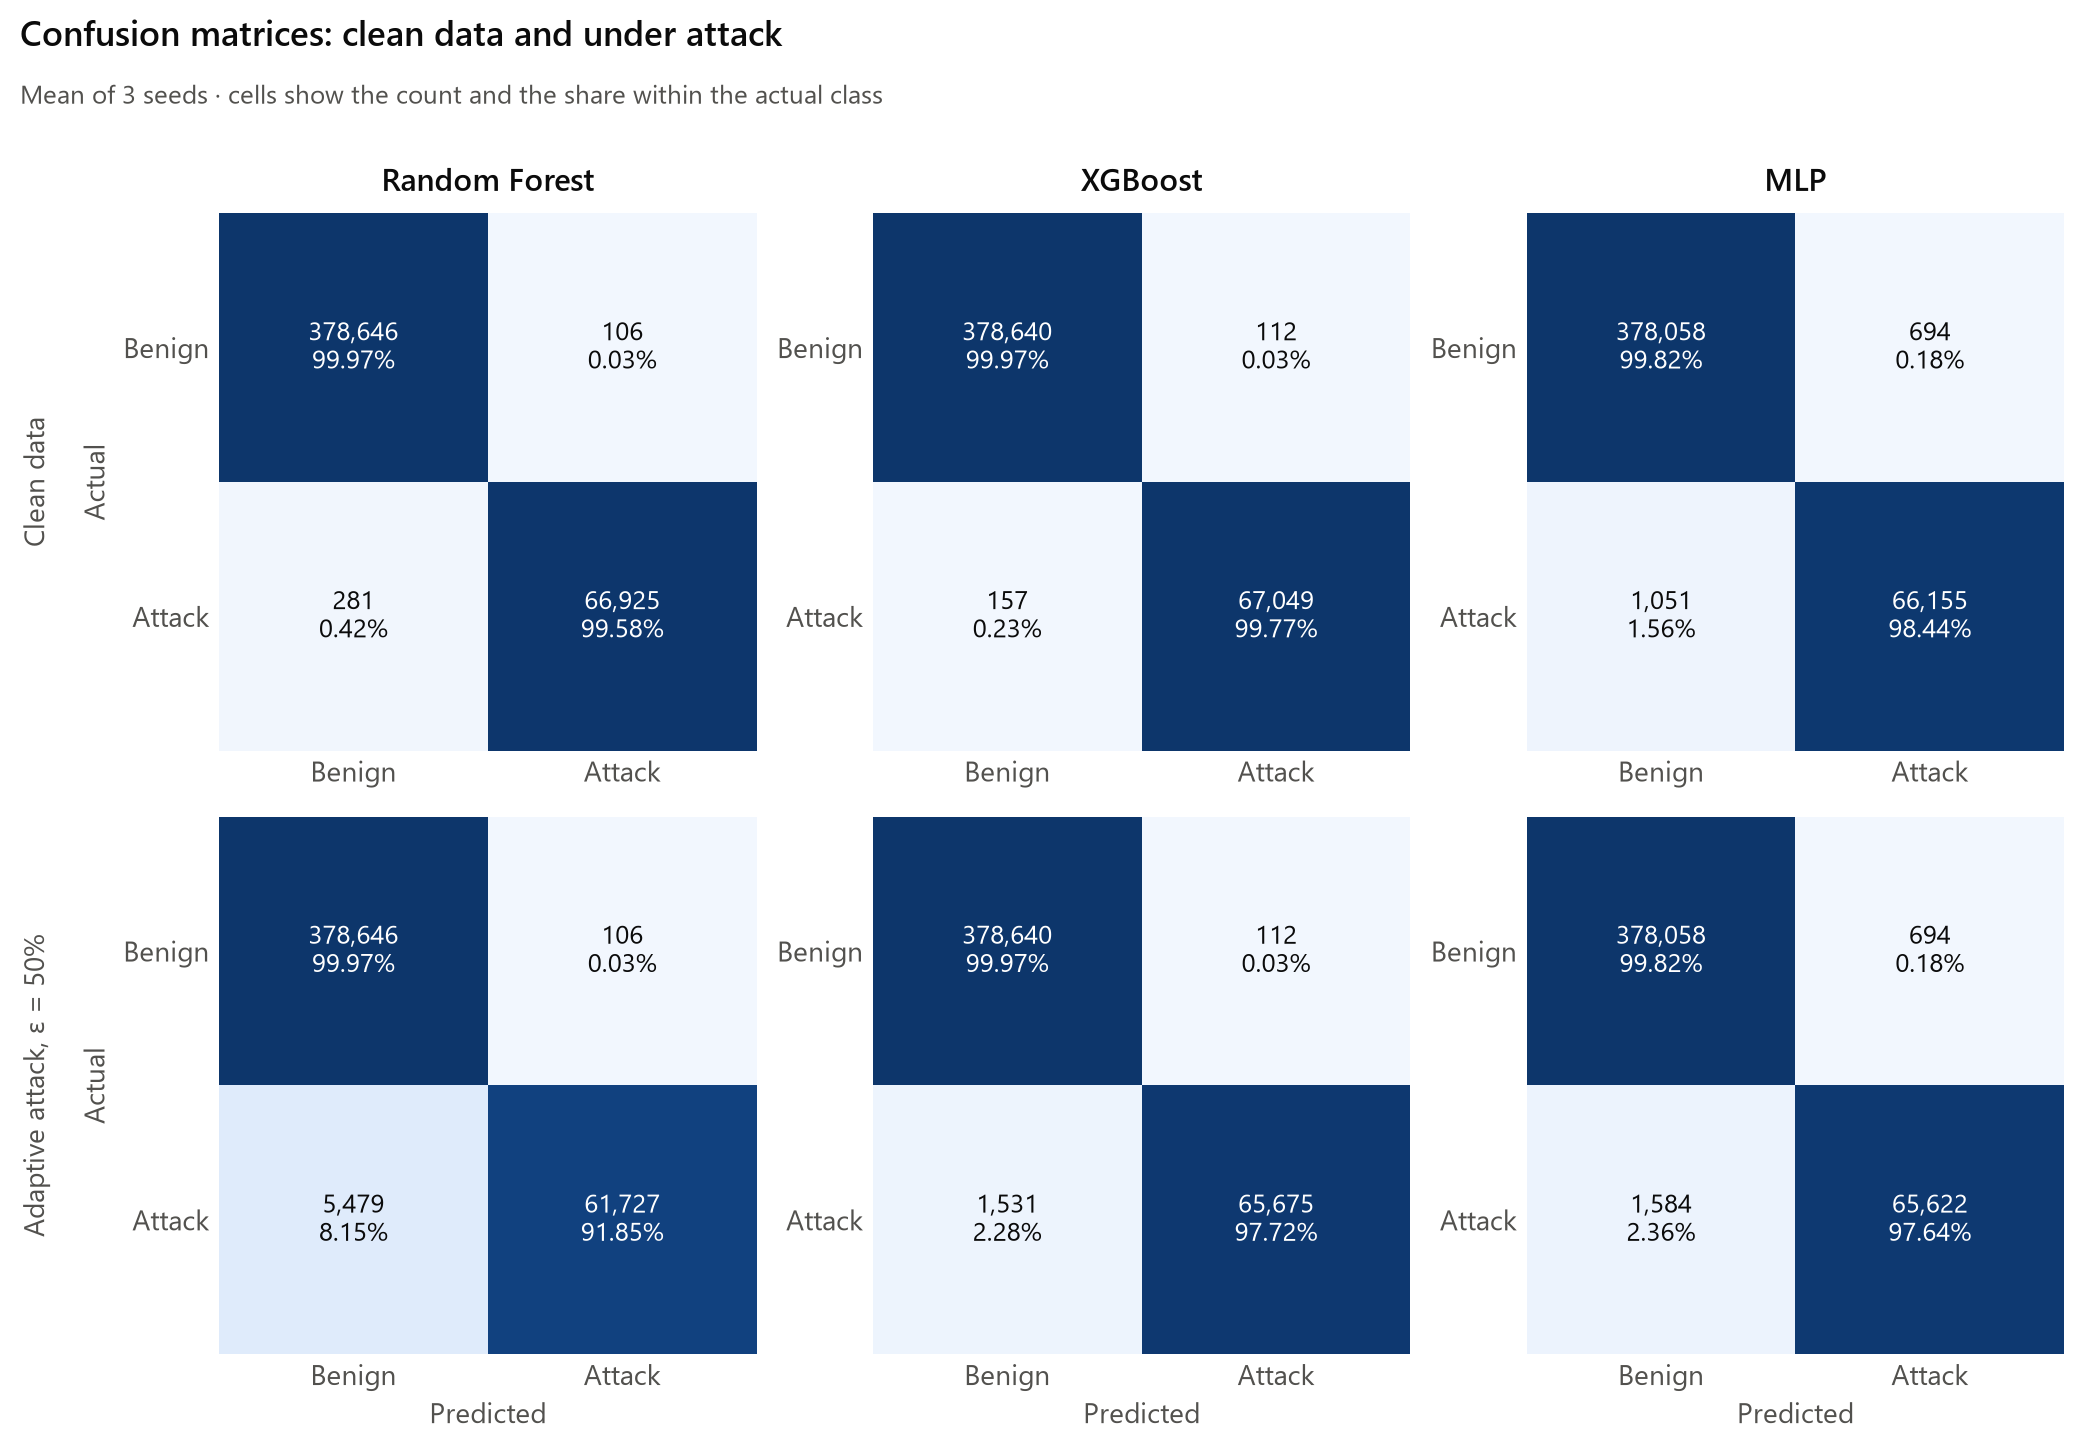
\includegraphics[width=0.78\textwidth]{02_confusion_matrix.png}
\caption{CIC-IDS2017 karışıklık matrisleri (3 seed ortalaması): üst satır temiz test verisi, alt satır uyarlamalı saldırgan altında (boyut+zaman, $\varepsilon=0.5$). Hücrelerde sayı ve gerçek sınıf içindeki pay gösterilmektedir.}
\label{fig:cm}
\end{figure*}

\subsection{Pertürbasyon duyarlılığı (Deney B)}
Şekil~\ref{fig:sens} uyarlamalı saldırgan altında Recall ve F1 değerlerinin bütçeyle değişimini göstermektedir. Random Forest'ın başarısı yalnızca boyut değiştirildiğinde bile $\varepsilon \geq 0.5$ seviyesinde belirgin biçimde düşmektedir; boyut ve zaman birlikte değiştirildiğinde $\varepsilon=1.0$'da Recall 0.813'e iner, kaçırılan saldırı sayısı 12\,581'e çıkar. Aynı bütçede XGBoost'un Recall değeri 0.968, MLP'ninki 0.954'tür.

Uyarlamalı saldırgan her senaryoda rastgele saldırgandan daha etkilidir. $\varepsilon=0.5$'te Random Forest'ın kaçırdığı saldırı sayısı rastgele saldırganla 2\,249, uyarlamalı saldırganla 5\,479'dur. Dolayısıyla aynı bütçeyle modelin skorunu sorgulayabilen bir saldırgan kaybı iki katından fazla artırabilmektedir.

Zaman pertürbasyonunda dikkat çekici bir örüntü gözlenmektedir: Random Forest ve XGBoost'un Recall değeri yalnızca \%5'lik bir gecikmeyle ani bir düşüş göstermekte, daha büyük bütçelerde ise neredeyse sabit kalmaktadır. Bunun nedenini incelemek için bütün saldırı akışları sabit \%5 geciktirilmiş ve XGBoost modeliyle (seed 42, 400\,000 eğitim örneği) değerlendirilmiştir. Tespitten kaçan 883 akışın 530'u DoS Slowhttptest (bu türün test kümesindeki akışlarının \%52.1'i), 328'i DoS slowloris (\%31.2) türündendir. Kaçan akışların medyan süresi 63.1~saniyedir. Yavaş DoS araçları sabit zamanlayıcılarla çalıştığından modeller bu saldırıları davranışlarından çok sabit bir süre imzasından tanımayı öğrenmiştir; küçük bir gecikme bu imzayı bozmaya yetmektedir.

\begin{figure*}[t]
\centering
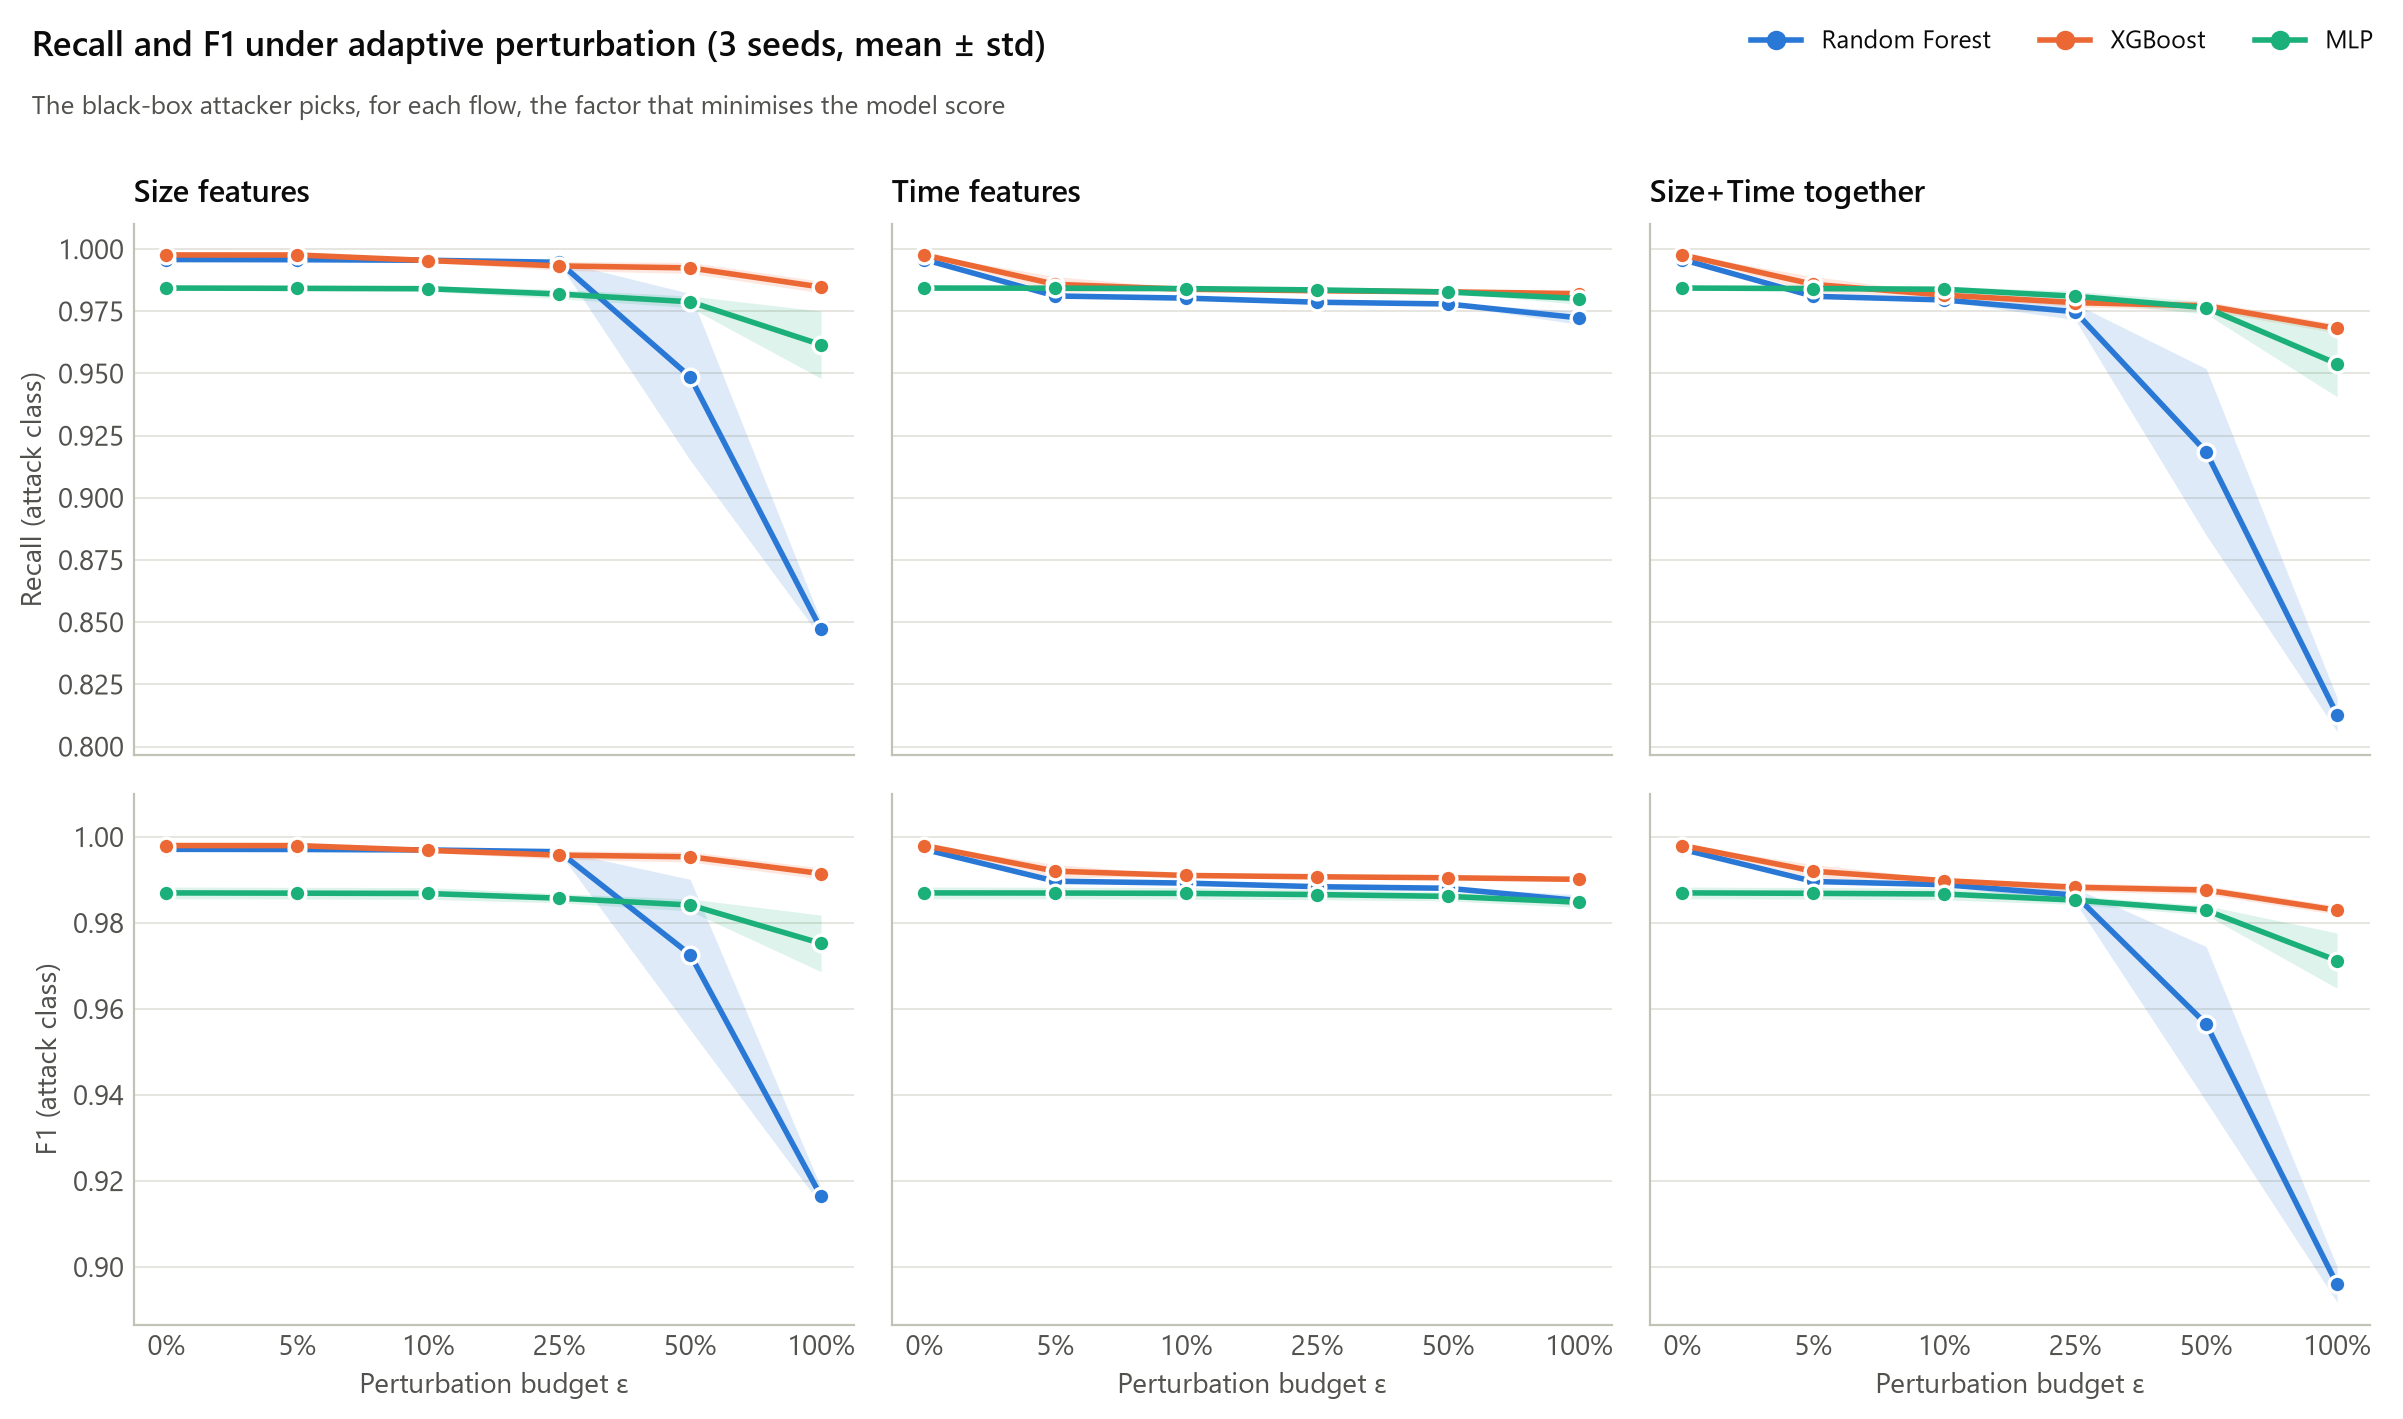
\includegraphics[width=0.9\textwidth]{04_sensitivity_adaptive.png}
\caption{CIC-IDS2017, uyarlamalı saldırgan: pertürbasyon bütçesine göre saldırı sınıfı Recall ve F1 değerleri (3 seed, ortalama $\pm$ std).}
\label{fig:sens}
\end{figure*}

\subsection{Model karşılaştırması (Deney C)}
Tablo~\ref{tab:robust} referans senaryodaki (uyarlamalı saldırgan, boyut ve zaman birlikte, $\varepsilon=0.5$) sonuçları vermektedir. Göreli F1 kaybına göre sıralama MLP $>$ XGBoost $>$ Random Forest şeklindedir. Ancak saldırı altındaki mutlak F1 değerinde XGBoost (0.9876) MLP'nin (0.9829) önündedir: MLP daha düşük bir başlangıç noktasından başladığı için daha az kaybetmektedir. ``En dayanıklı model'' sorusunun cevabı bu nedenle kullanılan ölçüte bağlıdır.

Güven aralıkları sıralamanın ne kadar kesin olduğunu da göstermektedir. 2017'de Random Forest'ın göreli kaybı seedler arasında belirgin biçimde değişmektedir (seed 42'de \%2.0, diğer iki seed'de \%5.0 ve \%5.3); bu nedenle \%95 GA geniştir ve sıfırı içermektedir. Dolayısıyla 2017'de yalnızca XGBoost ile MLP arasındaki fark seed değişkenliğinden ayırt edilebilmektedir; Random Forest'ın aralığı diğer iki modelinkiyle çakışmaktadır. 2018'de ise üç modelin aralıkları birbirinden tamamen ayrıktır ve sıralama nettir.

\begin{table*}[t]
\caption{Uyarlamalı saldırgan, boyut+zaman, $\varepsilon = 0.5$ (3 seed, ortalama). GA: seedler üzerinden t dağılımına dayalı \%95 güven aralığı. Kaçırılan artış: test kümesindeki saldırılara oranla yüzde puan.}
\label{tab:robust}
\centering
\small
\begin{tabular}{llccccc}
\toprule
Veri seti & Model & F1 (temiz $\rightarrow$ saldırı) & Göreli F1 düşüşü (\%) & \%95 GA & Kaçırılan artış (puan) & Sıra \\
\midrule
\multirow{3}{*}{CIC-IDS2017} & Random Forest & 0.9971 $\rightarrow$ 0.9565 & 4.07 & [$-$0.45, 8.59] & 7.73 & 3 \\
 & XGBoost & 0.9980 $\rightarrow$ 0.9876 & 1.04 & [0.79, 1.28] & 2.04 & 2 \\
 & MLP & 0.9870 $\rightarrow$ 0.9829 & 0.41 & [0.07, 0.75] & 0.79 & 1 \\
\midrule
\multirow{3}{*}{CSE-CIC-IDS2018} & Random Forest & 0.9233 $\rightarrow$ 0.8549 & 7.40 & [5.29, 9.51] & 11.47 & 2 \\
 & XGBoost & 0.9369 $\rightarrow$ 0.9307 & 0.66 & [0.39, 0.93] & 1.09 & 1 \\
 & MLP & 0.9322 $\rightarrow$ 0.7554 & 18.97 & [18.56, 19.39] & 26.79 & 3 \\
\bottomrule
\end{tabular}
\end{table*}

Kayıp metrikler arasında eşit dağılmamaktadır. Random Forest için referans senaryoda göreli düşüş Recall'da \%7.77, F1'de \%4.07, doğrulukta \%1.17, kesinlikte ise yalnızca \%0.01'dir. Kesinliğin değişmemesi tasarımın doğal bir sonucudur: normal trafiğe dokunulmadığı için yanlış alarm sayısı artmamakta, yalnızca kaçırılan saldırı sayısı artmaktadır. Doğruluğun az değişmesi ise sınıf dengesizliğinden kaynaklanmaktadır. Dikkat çekici olan, PR-AUC'nin neredeyse hiç değişmemesidir: $\varepsilon=1.0$'da Random Forest'ın Recall değeri 0.813'e düşerken PR-AUC 0.9970'te kalmaktadır.

\textbf{H1.} Düzeltme yapılmadan 18 kombinasyonun 17'sinde $\varepsilon$ ile hem Recall hem F1 arasında negatif ve anlamlı bir korelasyon bulunmaktadır. Holm düzeltmesinden sonra bu sayı 14'e inmektedir. Desteklenmeyen dört kombinasyonun tamamı MLP'ye aittir: rastgele saldırganla zaman grubu düzeltmeden önce de desteklenmemekteydi; diğer üçü (rastgele boyut, rastgele boyut+zaman ve uyarlamalı zaman) ise düzeltmeyle desteğini yitirmektedir. Bu üç kombinasyonda Recall'daki düşüş anlamlı kalırken F1'deki düşüş anlamlılığını yitirmektedir. Ağaç tabanlı modellerin 12 kombinasyonunun tamamında H1 düzeltmeden sonra da desteklenmektedir.

\subsection{Özellik önemi ve ablasyon (Deney D)}
Boyut özellikleri toplam önemin Random Forest'ta \%68.9'unu, XGBoost'ta \%76.9'unu oluşturmaktadır. Ablasyon sonuçları (Tablo~\ref{tab:ablation}, Şekil~\ref{fig:ablation}) dayanıklılığın kaynağını göstermektedir. Boyut grubu çıkarıldığında Random Forest'ın saldırı altındaki kaybı yaklaşık \%60 azalmaktadır ($\Delta F1$: $-0.055 \rightarrow -0.021$); saldırganın değiştirdiği gruba bağımlılığın azalması kaybı da azaltmaktadır. Saldırganın değiştiremediği sayaç ve protokol özellikleri (paket sayıları, TCP bayrakları, pencere boyutu) çıkarıldığında ise kayıp en fazla artmaktadır (RF: $-0.083$, XGBoost: $-0.050$). Zaman grubu çıkarıldığında XGBoost'un kaybı dört katına çıkmaktadır ($-0.011 \rightarrow -0.044$), çünkü model bu durumda saldırganın değiştirebildiği boyut özelliklerine daha fazla dayanmaktadır. MLP'nin kaybı bütün varyantlarda küçük kalmaktadır.

\begin{table}[t]
\caption{Özellik grubu ablasyonu, CIC-IDS2017: saldırı altında $\Delta F1$ (uyarlamalı, boyut+zaman, $\varepsilon = 0.5$; 3 seed). Modeller hesaplama süresi nedeniyle 400\,000 örnekle yeniden eğitilmiştir; bu nedenle ``Yok'' satırı Tablo~\ref{tab:robust}'teki tam veri sonuçlarından biraz farklıdır.}
\label{tab:ablation}
\centering
\begin{tabular}{lccc}
\toprule
Çıkarılan grup & RF & XGBoost & MLP \\
\midrule
Yok (tüm özellikler) & $-0.055$ & $-0.011$ & $-0.005$ \\
Boyut & $-0.021$ & $-0.007$ & $-0.008$ \\
Zaman & $-0.061$ & $-0.044$ & $-0.005$ \\
Hız & $-0.050$ & $-0.012$ & $-0.007$ \\
Sayaç/Protokol & $-0.083$ & $-0.050$ & $-0.005$ \\
\bottomrule
\end{tabular}
\end{table}

\begin{figure*}[t]
\centering
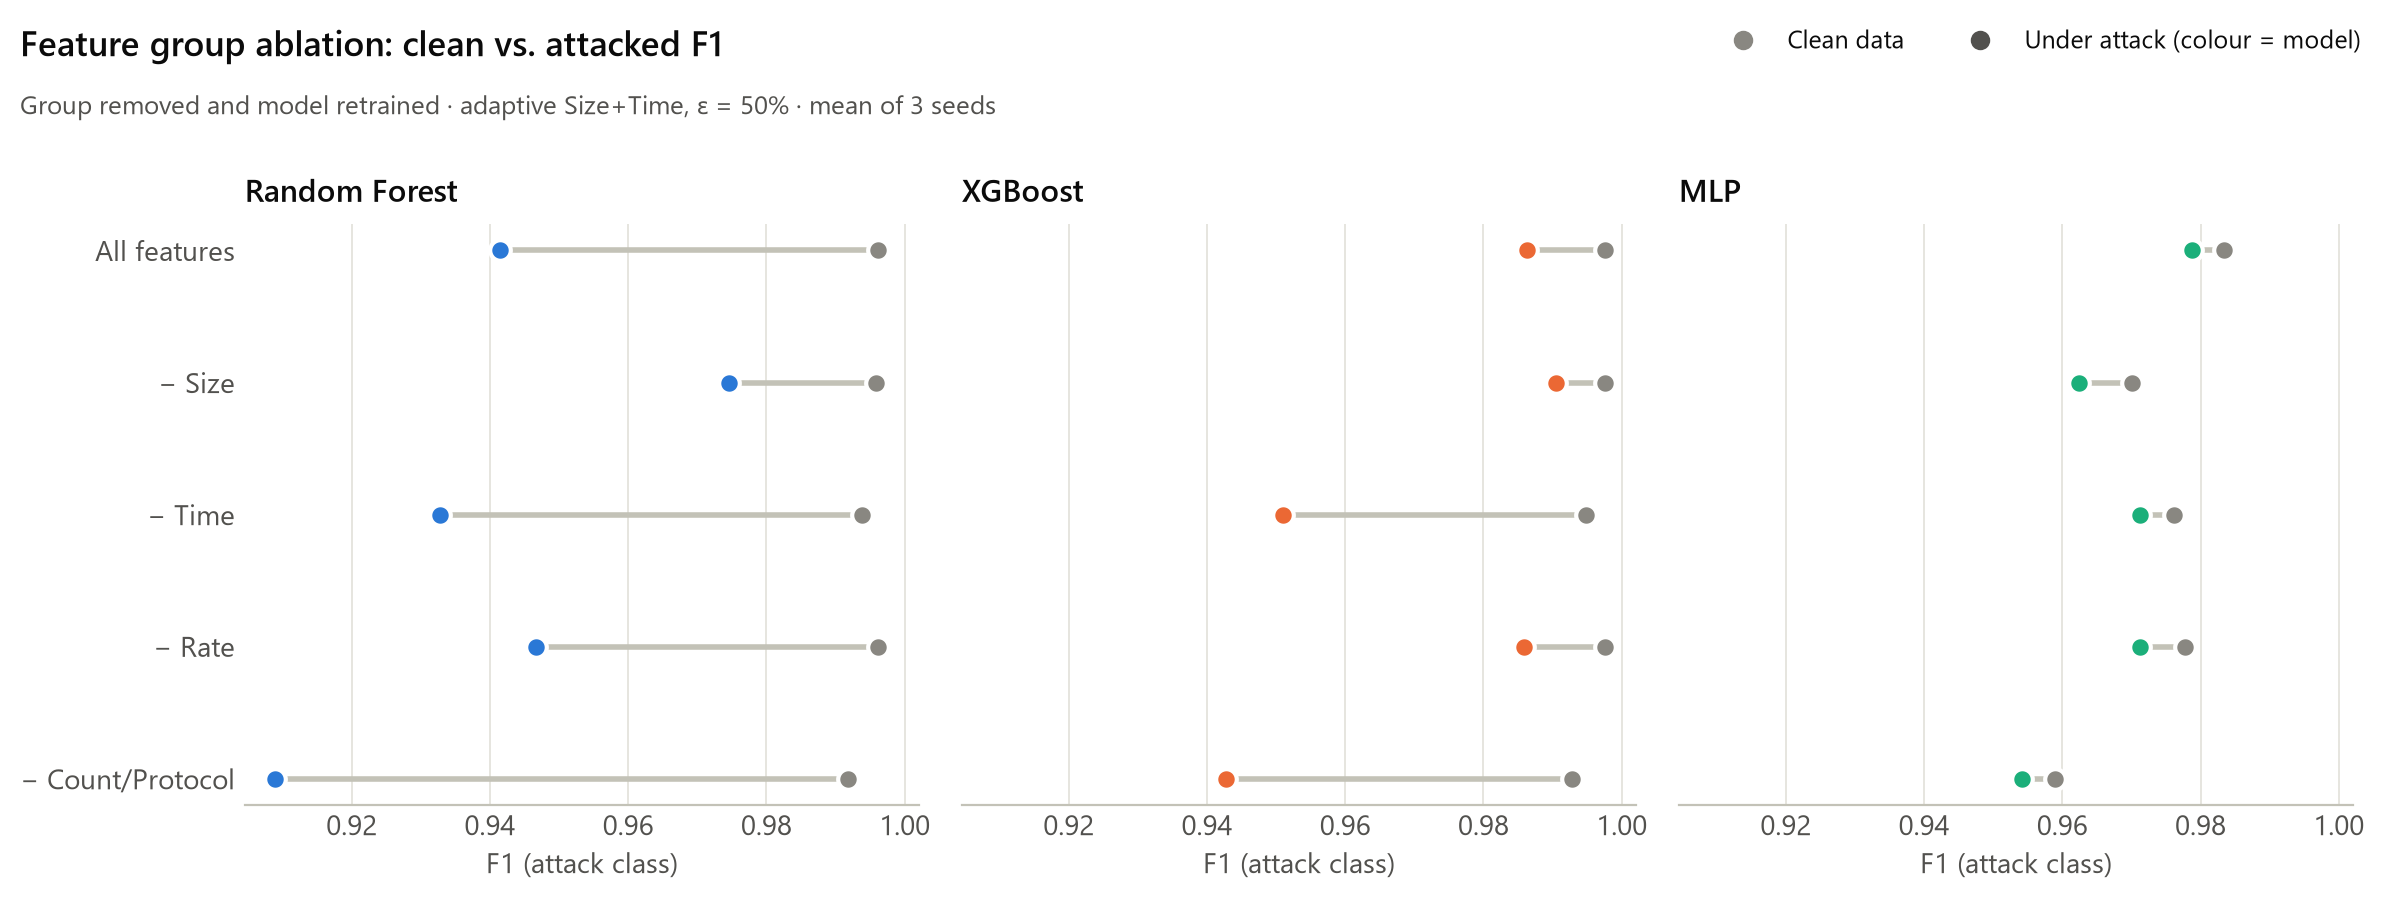
\includegraphics[width=0.85\textwidth]{09_ablation.png}
\caption{Özellik grubu ablasyonu: gri nokta temiz veride, renkli nokta saldırı altındaki F1 değeri (uyarlamalı, boyut+zaman, $\varepsilon=0.5$). Her varyantta grup çıkarılıp model yeniden eğitilmiştir.}
\label{fig:ablation}
\end{figure*}

\subsection{CSE-CIC-IDS2018 ile karşılaştırma}
2018'de üç modelin temiz F1 değeri 0.923--0.937 aralığındadır ve Recall yaklaşık 0.88'dir. Saldırı türü bazındaki analiz (Tablo~\ref{tab:types}) bu farkın neredeyse tamamının \emph{Infilteration} sınıfından geldiğini göstermektedir: bu sınıfta Recall \%0.8--7.1 arasındadır ve temiz veride kaçırılan saldırıların \%95.7--98.5'i bu sınıfa aittir. Infilteration hariç tutulduğunda Recall 0.994--0.998'e çıkmakta ve 2017 ile aynı düzeye gelmektedir.

\begin{table}[t]
\caption{CSE-CIC-IDS2018, saldırı türü bazında Recall (seed 42): temiz / uyarlamalı boyut saldırısı, $\varepsilon = 0.5$}
\label{tab:types}
\centering
\footnotesize
\setlength{\tabcolsep}{3pt}
\begin{tabular}{lrccc}
\toprule
Saldırı türü & Test & RF & XGBoost & MLP \\
\midrule
DDoS-HOIC & 15\,550 & 0.998 / 0.998 & 1.000 / 1.000 & 1.000 / 1.000 \\
DoS-Hulk & 13\,135 & 1.000 / 1.000 & 1.000 / 1.000 & 1.000 / 1.000 \\
Bot & 8\,503 & 0.992 / 0.992 & 0.994 / 0.994 & 0.975 / 0.039 \\
Infilteration & 6\,099 & 0.071 / 0.051 & 0.047 / 0.040 & 0.008 / 0.008 \\
SSH-Bruteforce & 5\,827 & 1.000 / 0.009 & 1.000 / 0.991 & 0.999 / 0.004 \\
DoS-GoldenEye & 2\,553 & 1.000 / 1.000 & 1.000 / 0.931 & 1.000 / 0.983 \\
\bottomrule
\end{tabular}
\end{table}

Saldırı altındaki sıralama 2018'de değişmektedir (Tablo~\ref{tab:robust}, Şekil~\ref{fig:cross}): XGBoost $>$ Random Forest $>$ MLP. MLP birinci sıradan son sıraya düşmekte, göreli F1 kaybı \%0.41'den \%18.97'ye çıkmaktadır. Tablo~\ref{tab:types} bunun nedenini göstermektedir: paketler \%50 büyütüldüğünde MLP Bot saldırılarının yalnızca \%3.9'unu, SSH-Bruteforce saldırılarının ise \%0.4'ünü tanıyabilmektedir; Random Forest'ın SSH-Bruteforce başarısı da \%0.9'a düşmektedir. XGBoost ise iki türü de tanımaya devam etmektedir. Bu iki tür 2018'deki saldırı akışlarının yaklaşık \%27'sini oluştururken 2017'deki karşılıkları (Bot ve SSH-Patator) yalnızca \%1.4'ünü oluşturmaktadır. H1 2018'de de 18 kombinasyonun 17'sinde desteklenmektedir. Holm düzeltmesinden sonra bu sayı 16'ya inmektedir; desteğini yitiren tek kombinasyon, rastgele saldırganla zaman pertürbasyonundaki XGBoost'tur. Bu senaryoda XGBoost'un kaybı zaten çok küçüktür.

\begin{figure*}[t]
\centering
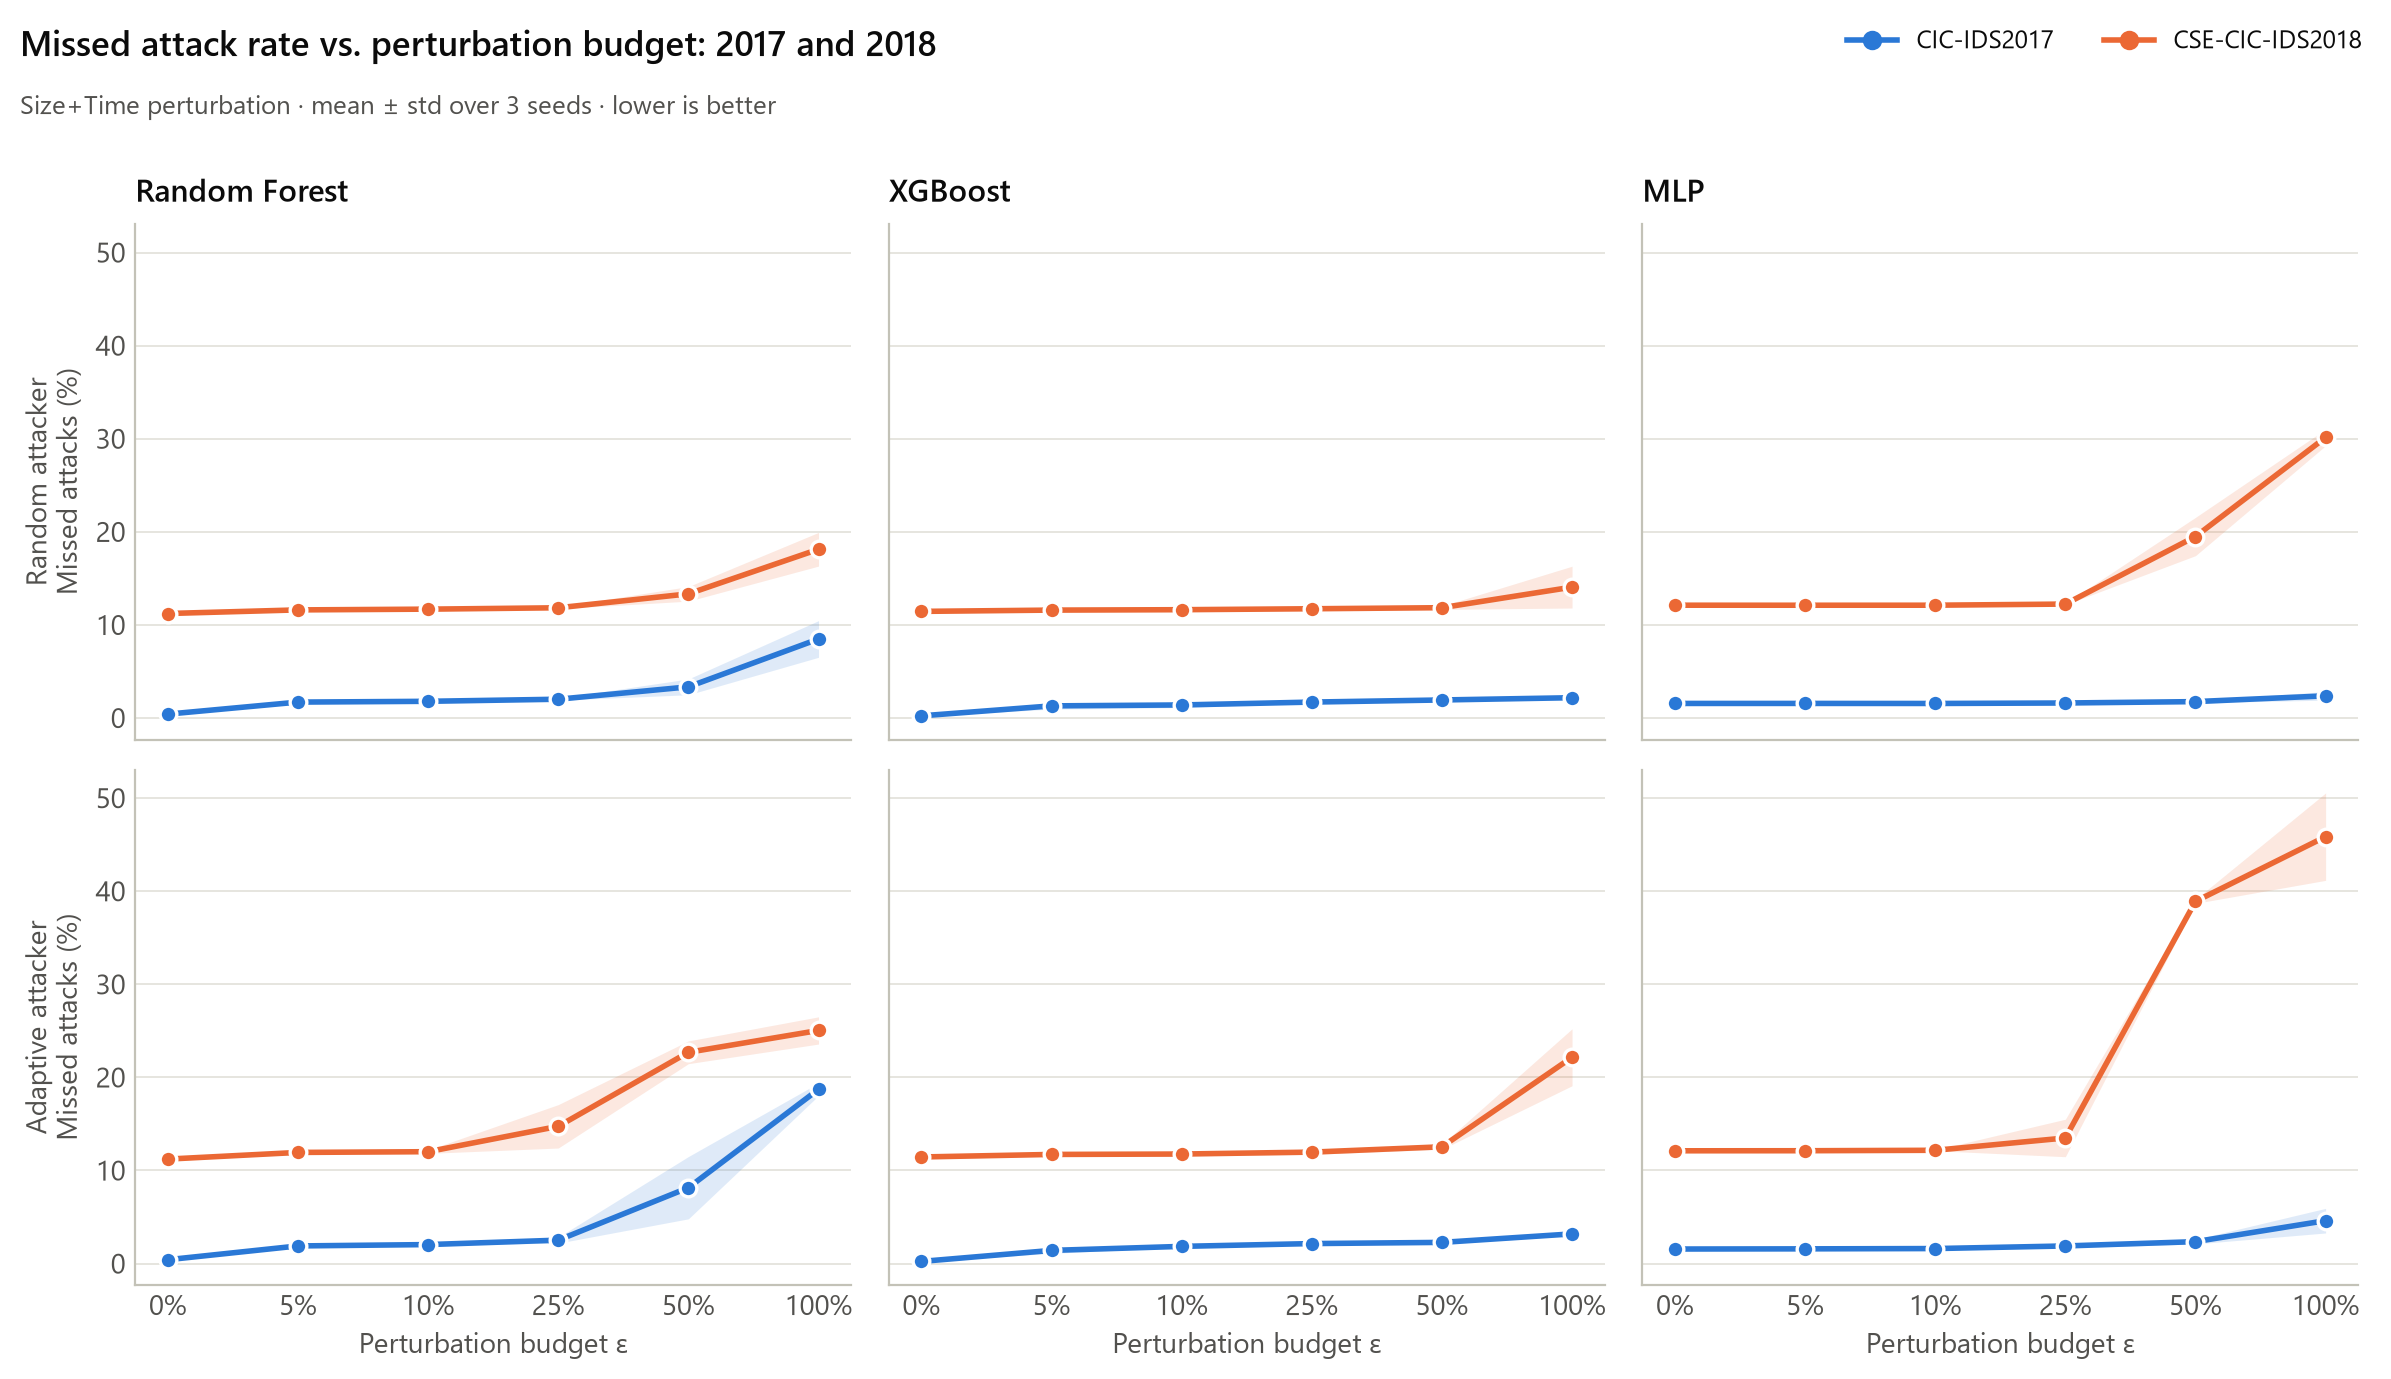
\includegraphics[width=0.9\textwidth]{K1_missed_attacks_comparison.png}
\caption{Boyut+zaman pertürbasyonunda kaçırılan saldırı oranı: CIC-IDS2017 ve CSE-CIC-IDS2018 (3 seed, ortalama $\pm$ std).}
\label{fig:cross}
\end{figure*}

\subsection{Karar eşiği ve kalibrasyon}
Temiz test verisinde üç model de iyi kalibre durumdadır; ECE değerleri 0.0002--0.0015 arasındadır. Platt ve isotonic yöntemleri Random Forest'ın ECE değerini yaklaşık üçte bire (0.00068 $\rightarrow$ 0.00016--0.00020), isotonic regression ise MLP'ninkini 0.00154'ten 0.00034'e indirmektedir; XGBoost'ta ve temperature scaling'de belirgin bir değişiklik gözlenmemektedir. Bu nedenle kalibrasyon sorunu saldırı altındaki kaybı açıklayacak büyüklükte değildir.

Eşik seçimi ise sonucu belirgin biçimde değiştirmektedir (Tablo~\ref{tab:threshold}, Şekil~\ref{fig:threshold}). Random Forest'ta saldırı altında kaçan saldırı sayısı sabit 0.5 eşiğiyle 5\,834 iken doğrulamada F1'i en yüksek yapan eşikle (yaklaşık 0.41) 2\,675'e, yanlış alarm oranını \%0.1 ile sınırlayan eşikle (yaklaşık 0.24) 1\,358'e inmektedir (\%77 azalma). Bunun bedeli, temiz veride yanlış alarm sayısının 112'den 360'a çıkmasıdır; bu değer normal trafiğin yaklaşık \%0.1'ine karşılık gelmektedir. Temiz F1 ise neredeyse değişmemektedir (0.9971 $\rightarrow$ 0.9965). Şekil~\ref{fig:threshold} bunun nedenini göstermektedir: saldırı altında Random Forest'ın Recall eğrisi 0.5 civarında hızla düşmekte, daha düşük eşiklerde ise temiz veriye yaklaşmaktadır. Uyarlamalı saldırgan Random Forest'ın skorunu 0.5'in hemen altına itebilmekte, ancak çok daha aşağı indirememektedir; skor ağaç oylarının oranı olduğundan birkaç ağacın kararını değiştirmek eşiği geçmeye yetmektedir. XGBoost'ta aynı politika kaçan saldırıları \%23 azaltmaktadır (1\,444 $\rightarrow$ 1\,106). MLP'de ise bu politika eşiği 0.5'in üzerine (yaklaşık 0.70) çıkarmakta ve kaybı artırmaktadır; bunun nedeni MLP'nin temiz veride zaten çok sayıda yanlış alarm üretmesidir.

Kalibre edilmiş olasılıkta 0.5 eşiğini kullanmak, ham skorda farklı bir eşik kullanmakla eşdeğerdir. Örneğin Random Forest'ta isotonic regression ile 0.5 eşiğinin sonucu, doğrulamadan seçilen F1-max eşiğinin sonucuyla aynıdır. Kalibrasyonun saldırı altındaki etkisi tamamen bu örtük eşik değişiminden kaynaklanmaktadır; olasılıkların daha iyi kalibre olması tek başına dayanıklılık sağlamamaktadır.

\begin{table}[t]
\caption{Eşik politikaları, CIC-IDS2017 (3 seed ortalaması). Eşikler yalnızca doğrulama verisiyle seçilmiştir. Saldırı: uyarlamalı, boyut+zaman, $\varepsilon = 0.5$.}
\label{tab:threshold}
\centering
\footnotesize
\setlength{\tabcolsep}{3pt}
\begin{tabular}{llcrccr}
\toprule
 & & & \multicolumn{2}{c}{Temiz} & \multicolumn{2}{c}{Saldırı altında} \\
\cmidrule(lr){4-5}\cmidrule(lr){6-7}
Model & Politika & Eşik & FP & F1 & F1 & FN \\
\midrule
\multirow{3}{*}{RF} & 0.5 & 0.50 & 112 & 0.9971 & 0.9537 & 5\,834 \\
 & F1-max & 0.41 & 168 & 0.9972 & 0.9784 & 2\,675 \\
 & FPR $\leq$ \%0.1 & 0.24 & 360 & 0.9965 & 0.9871 & 1\,358 \\
\midrule
\multirow{3}{*}{XGBoost} & 0.5 & 0.50 & 120 & 0.9980 & 0.9883 & 1\,444 \\
 & F1-max & 0.55 & 119 & 0.9979 & 0.9877 & 1\,518 \\
 & FPR $\leq$ \%0.1 & 0.13 & 345 & 0.9972 & 0.9891 & 1\,106 \\
\midrule
\multirow{3}{*}{MLP} & 0.5 & 0.50 & 747 & 0.9867 & 0.9822 & 1\,631 \\
 & F1-max & 0.55 & 616 & 0.9874 & 0.9819 & 1\,789 \\
 & FPR $\leq$ \%0.1 & 0.70 & 393 & 0.9825 & 0.9761 & 2\,756 \\
\bottomrule
\end{tabular}
\end{table}

\begin{figure*}[t]
\centering
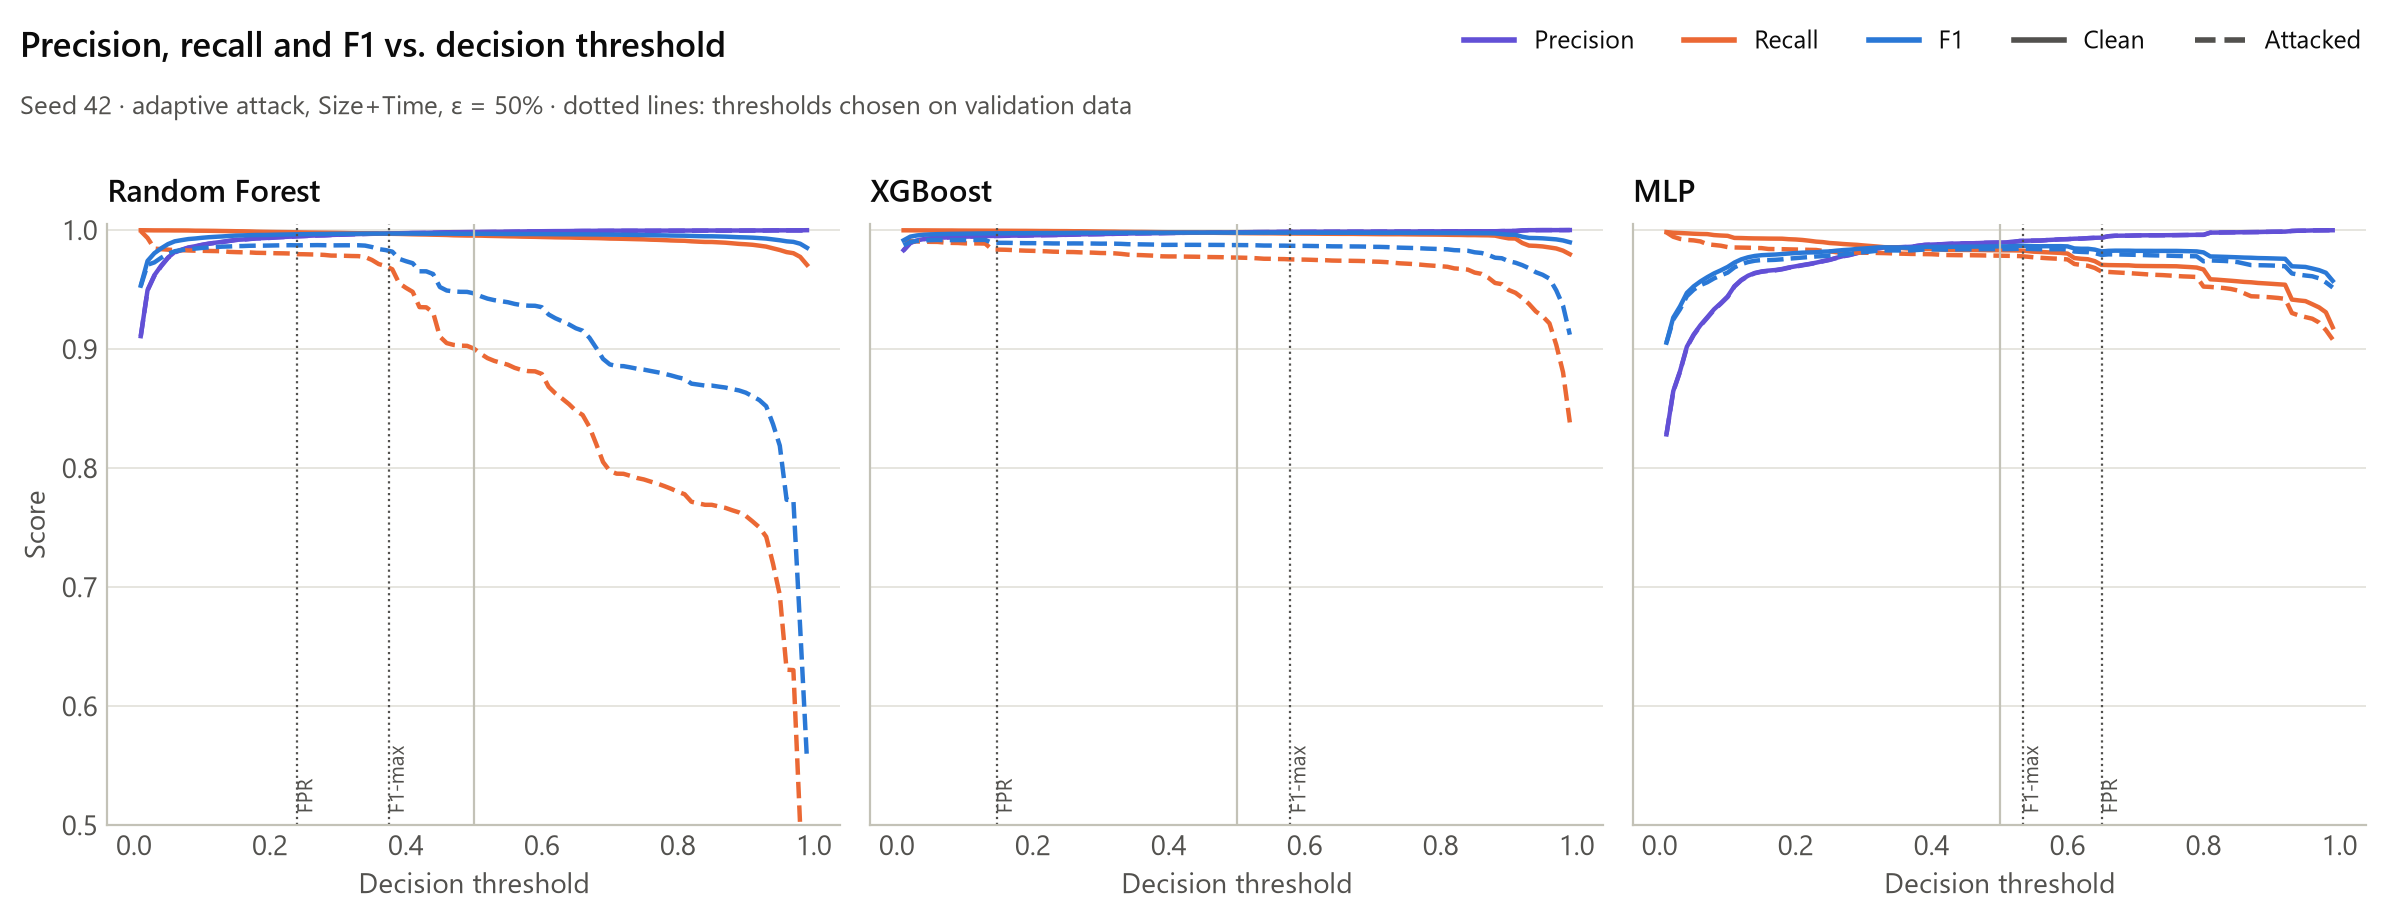
\includegraphics[width=0.9\textwidth]{C2_threshold_curves.png}
\caption{CIC-IDS2017, seed 42: karar eşiğine göre Precision, Recall ve F1; düz çizgi temiz veriyi, kesikli çizgi uyarlamalı saldırı altındaki sonucu (boyut+zaman, $\varepsilon=0.5$) göstermektedir. Noktalı dikey çizgiler doğrulama verisiyle seçilen eşiklerdir.}
\label{fig:threshold}
\end{figure*}

\subsection{Hata analizi}
Saldırı altında kaçan akışların kaynağı modele göre değişmektedir (CIC-IDS2017, seed 42, eşik 0.5). Random Forest'ta kaçan akışların \%72'si DDoS türündendir (bu türde Recall 0.9995 $\rightarrow$ 0.813). XGBoost'ta ise kaçanların çoğunluğu yavaş DoS türlerindedir (Slowhttptest \%38, slowloris \%22) ve DDoS'ta Recall 0.986'da kalmaktadır. MLP'nin saldırı altındaki kaybı küçüktür, ancak model bazı türleri temiz veride bile tanıyamamaktadır: Web Attack--Brute Force (Recall 0.075), XSS (0.028) ve Bot (0.48). MLP'nin temiz verideki yüksek FN sayısının kaynağı bu türlerdir. Somut bir örnek saldırganın etkisini açıkça göstermektedir: ileri yönde hiç veri taşımayan bir DoS Slowhttptest akışının süresi 63.1 saniyeden 73.7 saniyeye uzatıldığında XGBoost'un verdiği saldırı olasılığı 0.93'ten 0.01'e düşmektedir.

Normal trafiğe dokunulmadığı için yanlış alarmlar saldırıdan etkilenmemektedir. Temiz veride yanlış alarm oranı ağaç modellerinde \%0.03, MLP'de \%0.18'dir. Yanlış alarmlar HTTPS (443) ve 8080 portlarında yoğunlaşmaktadır; örneğin Random Forest'ın yanlış alarmlarının \%58'i port 443'ten gelirken bu port normal trafiğin \%24'ünü oluşturmaktadır. Üç modelin 50 yanlış alarmı ortaktır; bu sayı ağaç modellerinin yanlış alarmlarının yaklaşık \%40--46'sına karşılık gelmektedir. Farklı karar mantığına sahip üç modelin aynı akışlarda yanılması, bu akışların bir kısmının saldırı trafiğine çok benzediğini ya da yanlış etiketlenmiş olabileceğini düşündürmektedir \cite{engelen2021}.

\subsection{Hesaplama maliyeti}
Tablo~\ref{tab:cost} her model için bir seed'deki eğitim ve Deney B değerlendirmesinin toplam süresini ve akış başına çıkarım süresini vermektedir (Intel Core i5-11400H, 16~GB RAM). Deney B süresine uyarlamalı saldırganın her bütçe için modele yaptığı 24 sorgu turu da dahildir. Random Forest hem eğitimde hem çıkarımda en pahalı modeldir. XGBoost, Random Forest'tan yaklaşık dört buçuk kat daha hızlı eğitilmektedir (25 ve 113 saniye) ve hem en hızlı hem en dayanıklı model olduğu için performans--maliyet açısından öne çıkmaktadır. MLP çıkarımda en hızlı modeldir. Üç model de saniyede yüz binlerce akışı değerlendirebildiğinden çıkarım süresi pratikte belirleyici değildir. 2017'deki bütün deneyler (ablasyon dahil) yaklaşık 32 dakika, 2018 deneyleri yaklaşık 18 dakika, eşik ve kalibrasyon analizi ise yaklaşık 13 dakika sürmüştür.

\begin{table}[t]
\caption{Hesaplama maliyeti: seed başına eğitim + Deney B süresi (saniye) ve CIC-IDS2017'de akış başına çıkarım süresi (3 seed ortalaması)}
\label{tab:cost}
\centering
\begin{tabular}{lccc}
\toprule
 & \multicolumn{2}{c}{Eğitim + Deney B (sn)} & Çıkarım \\
\cmidrule(lr){2-3}
Model & 2017 & 2018 & ($\mu$s/akış) \\
\midrule
Random Forest & 161 & 146 & 1.54 \\
XGBoost & 66 & 55 & 0.79 \\
MLP & 100 & 55 & 0.19 \\
\bottomrule
\end{tabular}
\end{table}

\section{Tartışma}

\emph{Hangi model en az kaybı yaşamıştır?} Bu sorunun tek bir cevabı yoktur. 2017'de göreli kayıpta MLP, saldırı altındaki mutlak başarıda XGBoost öndedir; 2018'de ise her iki ölçütte de XGBoost öndedir. Random Forest ortalamada iki veri setinde de en büyük kayıplardan birini yaşamaktadır, ancak 2017'de bu kayıp seedler arasında belirgin biçimde değişmektedir. Random Forest'ın bu kırılganlığı, ağaç topluluklarının eşik tabanlı kararlarının küçük değişikliklerle aşılabildiğini gösteren önceki çalışmalarla uyumludur \cite{kantchelian2016}. XGBoost'un daha istikrarlı olmasının olası bir nedeni, sınırlı derinlikteki ağaçların birbirinin hatasını düzelterek kararı tek bir özelliğe daha az bağlamasıdır; ancak bu açıklama bu çalışmada doğrudan sınanmamıştır.

\emph{Performans kaybı en çok hangi metrikte görülmüştür?} Kayıp en çok Recall'da görülmektedir. PR-AUC ve ROC-AUC'nin neredeyse sabit kalması, pertürbasyonun saldırı akışlarını sıralamada normal trafiğin arasına karıştırmadığını, yalnızca skorlarını 0.5 eşiğinin altına ittiğini göstermektedir. Eşik analizi bu yorumu doğrulamaktadır: Random Forest'ta eşik yalnızca doğrulama verisiyle ve bir yanlış alarm bütçesine göre seçildiğinde saldırı altında kaçan saldırılar \%77 azalmakta, göreli F1 kaybı \%4.4'ten \%0.9'a inmektedir. Uyarlamalı saldırgan zaten skoru en aza indirdiği için bu kazanç saldırganın eşiği bilmemesinden değil, sınırlı bütçesiyle skoru eşiğin çok altına indirememesinden kaynaklanmaktadır. Bu nedenle 2017'deki dayanıklılık sıralamasının önemli bir kısmı sabit 0.5 eşiğine bağlıdır: yanlış alarm bütçesine göre seçilen eşiklerle saldırı altındaki F1 değerleri Random Forest için 0.9871, XGBoost için 0.9891 ve MLP için 0.9761'dir. Başka bir deyişle Random Forest ile XGBoost arasındaki fark büyük ölçüde kapanmaktadır. Kalibrasyon ise olasılıkların sırasını değiştirmediği için yalnızca örtük bir eşik değişikliği olarak etki etmektedir. Bu bulgular, IDS'lerin dayanıklılığı raporlanırken eşik seçiminin de değerlendirmenin bir parçası olması gerektiğine işaret etmektedir. Bununla birlikte daha güçlü bir saldırgan skorları daha da aşağı indirebileceğinden eşik ayarı tek başına bir savunma olarak görülmemelidir.

\emph{Hangi model hangi senaryoda tercih edilmelidir?} Sabit eşikle çalışan ve saldırı türü bileşiminin bilinmediği bir ortamda XGBoost en güvenli seçenektir: iki veri setinde de en düşük ya da ona yakın kayba sahiptir, en hızlı eğitilen modeldir ve eşik değişikliğine en az duyarlı olandır. Eşiğin doğrulama verisiyle ve bir yanlış alarm bütçesine göre ayarlanabildiği bir ortamda Random Forest da XGBoost'a yakın bir dayanıklılık göstermektedir, ancak eğitimi ve çıkarımı daha maliyetlidir. MLP çıkarımda en hızlı modeldir; ancak web saldırıları ve Bot gibi az örnekli türleri temiz veride bile tanıyamamakta, 2018'de küçük paket boyutlu saldırılara karşı çok kırılgan kalmakta ve ağaç modellerinin yaklaşık altı katı yanlış alarm üretmektedir. Bu nedenle tek başına kullanılması önerilmemektedir.

\emph{Bazı özellik gruplarındaki değişiklikler diğerlerinden daha mı etkilidir?} Boyut ve zamanın birlikte değiştirilmesi her durumda en etkili senaryodur. 2017'de Random Forest boyuta, XGBoost zamana daha duyarlıdır; 2018'de ise kaybın neredeyse tamamı boyut pertürbasyonundan gelmektedir. Ablasyon, saldırganın değiştiremediği özelliklerin bir çapa işlevi gördüğünü göstermektedir. Buradan çıkan pratik sonuç, değiştirilmesi güç özelliklere daha fazla dayanan modellerin evasion saldırılarına karşı daha dayanıklı olacağıdır.

\emph{Yanlış negatif sayısı nasıl değişmiştir?} Referans senaryoda kaçırılan saldırı sayısı Random Forest'ta 19.5 kat (281 $\rightarrow$ 5\,479), XGBoost'ta 9.8 kat (157 $\rightarrow$ 1\,531), MLP'de 1.5 kat (1\,051 $\rightarrow$ 1\,584) artmaktadır. Bir IDS için bu en maliyetli hata türüdür, çünkü kaçırılan bir saldırı hiçbir alarm üretmez.

\emph{Sonuçlar gerçek ağ ortamına ne ölçüde genellenebilir?} İki bulgu genelleme konusunda temkinli olmayı gerektirmektedir. Birincisi, yavaş DoS örneği modellerin bir kısım saldırıyı davranışlarından çok veri setine özgü sabit bir imzadan tanıdığını göstermektedir; bu, laboratuvarda üretilmiş veri setleri için daha önce dile getirilmiş bir endişedir \cite{sommer2010,arp2022}. İkincisi, dayanıklılık sıralamasının veri setleri arasında değişmesi, bir modelin dayanıklılığının yalnızca modele değil saldırı türlerinin bileşimine de bağlı olduğunu göstermektedir. 2018'deki Infilteration örneği ise düşük bir başarının modelden çok etiket kalitesini yansıtabileceğini ortaya koymaktadır; bu durum, iki veri setindeki etiketleme hatalarını raporlayan çalışmalarla uyumludur \cite{engelen2021,liu2022}.

\section{Geçerlilik Tehditleri ve Sınırlılıklar}

\emph{Özellik uzayında saldırı.} Paketler yeniden üretilmemiş, CICFlowMeter'ın çıkardığı özellikler doğrudan değiştirilmiştir. Paket düzeyindeki veri olmadan yeniden hesaplanamayan çift yönlü dağılım özellikleri (paket uzunluğu standart sapması ve varyansı, en küçük paket uzunluğu) sabit tutulmuştur. Zaman pertürbasyonu akışın tamamının orantılı olarak yavaşladığını varsaymaktadır; gerçekte gecikme yalnızca ileri yöndeki paketlere eklenir.

\emph{Saldırganın gücü.} Uyarlamalı saldırgan modelin olasılık çıktısını sınırsız sorgulayabildiği varsayımıyla çalışmaktadır. Gerçek bir IDS çoğunlukla yalnızca alarm bilgisi verir ve çok sayıda sorgu kendi başına şüphe uyandırabilir. Bu nedenle uyarlamalı saldırganın sonuçları bir üst sınır, rastgele saldırganın sonuçları ise bir alt sınır olarak okunmalıdır.

\emph{Saldırının işlevselliği.} Dolgu ve gecikmenin saldırının amacını (ör. DoS etkisini veya brute-force hızını) ne ölçüde azalttığı ölçülmemiştir. Bir akışın tespitten kaçması saldırının hâlâ başarılı olduğu anlamına gelmez.

\emph{Veri setleri.} Her iki veri seti de laboratuvar ortamında üretilmiştir. Rastgele bölme, aynı saldırı oturumundan gelen benzer akışları hem eğitim hem test kümesine yerleştirebilir ve baseline sonuçlarını iyimser gösterebilir. 2018 verisinin \%30'luk bir örneği kullanılmış, bir gün dışarıda bırakılmış ve ablasyon 2018 için tekrarlanmamıştır.

\emph{Model seçimi ve eşik.} Hiperparametre araması yapılmamıştır; sonuçlar bu nedenle modellerin en iyi ayarlanmış hâllerini değil, makul varsayılan ayarlarını yansıtmaktadır. Ana deneylerde karar eşiği 0.5'te sabit tutulmuştur. Eşik ve kalibrasyon analizi yalnızca CIC-IDS2017'de ve referans saldırı senaryosunda yapılmıştır; uyarlamalı saldırgan dört kademeli bir ızgarayla sınırlı olduğundan daha güçlü bir saldırgana karşı eşik ayarının kazancı daha küçük olabilir.

\emph{İstatistiksel güç.} Her deney yalnızca üç seed ile tekrarlanmıştır. Bu sayı ortalama ve standart sapma raporlamak için yeterli olmakla birlikte güven aralıklarını genişletmektedir; özellikle 2017'de Random Forest'ın diğer modellerden farkı bu nedenle istatistiksel olarak ayırt edilememektedir.

Bütün bu nedenlerle sonuçlar, modellerin kısıtlı pertürbasyonlar karşısındaki göreli kırılganlığının bir ölçüsü olarak okunmalı; gerçek bir saldırganın bu sistemleri aşabileceğinin kesin kanıtı olarak yorumlanmamalıdır.

\section{Sonuç}

Bu çalışmada üç IDS modelinin gerçekçi ağ kısıtlarını koruyan evasion saldırıları karşısındaki dayanıklılığı iki veri setinde incelenmiştir. Pertürbasyon bütçesi arttıkça saldırı sınıfındaki Recall ve F1 değerleri düşmektedir; H1 her iki veri setinde de 18 kombinasyonun 17'sinde desteklenmekte ve CIC-IDS2017'de ağaç tabanlı modellerin bütün senaryolarında çoklu karşılaştırma düzeltmesinden sonra da geçerliliğini korumaktadır. Kayıp Recall'da yoğunlaşmakta, sıralama kalitesi ise büyük ölçüde korunmaktadır. Eşik analizi bu kaybın önemli bir kısmının skorların sabit 0.5 eşiğinin hemen altına inmesinden kaynaklandığını göstermektedir: eşik yalnızca doğrulama verisiyle seçildiğinde Random Forest'ın saldırı altında kaçırdığı saldırılar \%77 azalmaktadır. Kalibrasyon ise olasılıkların sırasını değiştirmediği için dayanıklılığı tek başına iyileştirmemektedir. Modeli sorgulayabilen bir saldırgan, aynı bütçeyle rastgele bir saldırgandan çok daha etkilidir. Saldırganın değiştiremediği özellikler dayanıklılığa en fazla katkıyı sağlamaktadır. Dayanıklılık sıralaması veri setine göre değişmektedir; iki veri setinde de istikrarlı kalan tek model XGBoost'tur. Gelecek çalışmalarda daha güçlü ve eşiği hedef alan saldırganların, pertürbe edilmiş örneklerle eğitimin (adversarial training) \cite{madry2018}, veri setleri arası değerlendirmenin ve paket düzeyinde, problem uzayında yapılan saldırılarla doğrulamanın ele alınması planlanmaktadır. Bütün kod, deney ayarları ve sonuç tabloları proje deposunda bulunmaktadır\footnote{\url{https://github.com/akkuzukayagulsumprojectcentre/Gulsum_Projects/tree/main/projects/Omer_Faruk_Sayin}}.

\begin{thebibliography}{99}

\bibitem{szegedy2014}
C. Szegedy, W. Zaremba, I. Sutskever, J. Bruna, D. Erhan, I. Goodfellow, and R. Fergus, ``Intriguing properties of neural networks,'' in \emph{Proc. Int. Conf. Learn. Represent. (ICLR)}, 2014.

\bibitem{goodfellow2015}
I. J. Goodfellow, J. Shlens, and C. Szegedy, ``Explaining and harnessing adversarial examples,'' in \emph{Proc. Int. Conf. Learn. Represent. (ICLR)}, 2015.

\bibitem{biggio2013}
B. Biggio, I. Corona, D. Maiorca, B. Nelson, N. Šrndić, P. Laskov, G. Giacinto, and F. Roli, ``Evasion attacks against machine learning at test time,'' in \emph{Proc. Eur. Conf. Mach. Learn. Knowl. Discov. Databases (ECML PKDD)}, 2013, pp. 387--402.

\bibitem{apruzzese2022}
G. Apruzzese, M. Andreolini, L. Ferretti, M. Marchetti, and M. Colajanni, ``Modeling realistic adversarial attacks against network intrusion detection systems,'' \emph{Digit. Threats: Res. Pract.}, vol. 3, no. 3, 2022.

\bibitem{biggio2018}
B. Biggio and F. Roli, ``Wild patterns: Ten years after the rise of adversarial machine learning,'' \emph{Pattern Recognit.}, vol. 84, pp. 317--331, 2018.

\bibitem{kantchelian2016}
A. Kantchelian, J. D. Tygar, and A. D. Joseph, ``Evasion and hardening of tree ensemble classifiers,'' in \emph{Proc. Int. Conf. Mach. Learn. (ICML)}, 2016, pp. 2387--2396.

\bibitem{chen2020}
J. Chen, M. I. Jordan, and M. J. Wainwright, ``HopSkipJumpAttack: A query-efficient decision-based attack,'' in \emph{Proc. IEEE Symp. Secur. Privacy (SP)}, 2020, pp. 1277--1294.

\bibitem{pierazzi2020}
F. Pierazzi, F. Pendlebury, J. Cortellazzi, and L. Cavallaro, ``Intriguing properties of adversarial ML attacks in the problem space,'' in \emph{Proc. IEEE Symp. Secur. Privacy (SP)}, 2020, pp. 1332--1349.

\bibitem{sheatsley2022}
R. Sheatsley, N. Papernot, M. J. Weisman, G. Verma, and P. McDaniel, ``Adversarial examples for network intrusion detection systems,'' \emph{J. Comput. Secur.}, vol. 30, no. 5, pp. 727--752, 2022.

\bibitem{alhajjar2021}
E. Alhajjar, P. Maxwell, and N. Bastian, ``Adversarial machine learning in network intrusion detection systems,'' \emph{Expert Syst. Appl.}, vol. 186, Art. no. 115782, 2021.

\bibitem{rosenberg2021}
I. Rosenberg, A. Shabtai, Y. Elovici, and L. Rokach, ``Adversarial machine learning attacks and defense methods in the cyber security domain,'' \emph{ACM Comput. Surv.}, vol. 54, no. 5, 2021.

\bibitem{madry2018}
A. Madry, A. Makelov, L. Schmidt, D. Tsipras, and A. Vladu, ``Towards deep learning models resistant to adversarial attacks,'' in \emph{Proc. Int. Conf. Learn. Represent. (ICLR)}, 2018.

\bibitem{niculescu2005}
A. Niculescu-Mizil and R. Caruana, ``Predicting good probabilities with supervised learning,'' in \emph{Proc. Int. Conf. Mach. Learn. (ICML)}, 2005, pp. 625--632.

\bibitem{platt1999}
J. Platt, ``Probabilistic outputs for support vector machines and comparisons to regularized likelihood methods,'' in \emph{Advances in Large Margin Classifiers}. Cambridge, MA, USA: MIT Press, 1999, pp. 61--74.

\bibitem{zadrozny2002}
B. Zadrozny and C. Elkan, ``Transforming classifier scores into accurate multiclass probability estimates,'' in \emph{Proc. ACM SIGKDD Int. Conf. Knowl. Discov. Data Min. (KDD)}, 2002, pp. 694--699.

\bibitem{guo2017}
C. Guo, G. Pleiss, Y. Sun, and K. Q. Weinberger, ``On calibration of modern neural networks,'' in \emph{Proc. Int. Conf. Mach. Learn. (ICML)}, 2017, pp. 1321--1330.

\bibitem{sharafaldin2018}
I. Sharafaldin, A. H. Lashkari, and A. A. Ghorbani, ``Toward generating a new intrusion detection dataset and intrusion traffic characterization,'' in \emph{Proc. Int. Conf. Inf. Syst. Secur. Privacy (ICISSP)}, 2018, pp. 108--116.

\bibitem{engelen2021}
G. Engelen, V. Rimmer, and W. Joosen, ``Troubleshooting an intrusion detection dataset: The CICIDS2017 case study,'' in \emph{Proc. IEEE Secur. Privacy Workshops (SPW)}, 2021, pp. 7--12.

\bibitem{liu2022}
L. Liu, G. Engelen, T. Lynar, D. Essam, and W. Joosen, ``Error prevalence in NIDS datasets: A case study on CIC-IDS-2017 and CSE-CIC-IDS-2018,'' in \emph{Proc. IEEE Conf. Commun. Netw. Secur. (CNS)}, 2022, pp. 254--262.

\bibitem{sommer2010}
R. Sommer and V. Paxson, ``Outside the closed world: On using machine learning for network intrusion detection,'' in \emph{Proc. IEEE Symp. Secur. Privacy (SP)}, 2010, pp. 305--316.

\bibitem{arp2022}
D. Arp, E. Quiring, F. Pendlebury, A. Warnecke, F. Pierazzi, C. Wressnegger, L. Cavallaro, and K. Rieck, ``Dos and don'ts of machine learning in computer security,'' in \emph{Proc. USENIX Secur. Symp.}, 2022, pp. 3971--3988.

\bibitem{chen2016}
T. Chen and C. Guestrin, ``XGBoost: A scalable tree boosting system,'' in \emph{Proc. ACM SIGKDD Int. Conf. Knowl. Discov. Data Min. (KDD)}, 2016, pp. 785--794.

\bibitem{pedregosa2011}
F. Pedregosa \emph{et al.}, ``Scikit-learn: Machine learning in Python,'' \emph{J. Mach. Learn. Res.}, vol. 12, pp. 2825--2830, 2011.

\end{thebibliography}

\end{document}
